\documentclass[]{article}
\usepackage{lmodern}
\usepackage{amssymb,amsmath}
\usepackage{ifxetex,ifluatex}
\usepackage{fixltx2e} % provides \textsubscript
\ifnum 0\ifxetex 1\fi\ifluatex 1\fi=0 % if pdftex
  \usepackage[T1]{fontenc}
  \usepackage[utf8]{inputenc}
\else % if luatex or xelatex
  \ifxetex
    \usepackage{mathspec}
  \else
    \usepackage{fontspec}
  \fi
  \defaultfontfeatures{Ligatures=TeX,Scale=MatchLowercase}
\fi
% use upquote if available, for straight quotes in verbatim environments
\IfFileExists{upquote.sty}{\usepackage{upquote}}{}
% use microtype if available
\IfFileExists{microtype.sty}{%
\usepackage{microtype}
\UseMicrotypeSet[protrusion]{basicmath} % disable protrusion for tt fonts
}{}
\usepackage[margin=1in]{geometry}
\usepackage{hyperref}
\hypersetup{unicode=true,
            pdftitle={Regime Switching and Technical Trading with Dynamic Bayesian Networks in High-Frequency Stock Markets},
            pdfauthor={Luis Damiano, Brian Peterson, Michael Weylandt},
            pdfborder={0 0 0},
            breaklinks=true}
\urlstyle{same}  % don't use monospace font for urls
\usepackage{graphicx,grffile}
\makeatletter
\def\maxwidth{\ifdim\Gin@nat@width>\linewidth\linewidth\else\Gin@nat@width\fi}
\def\maxheight{\ifdim\Gin@nat@height>\textheight\textheight\else\Gin@nat@height\fi}
\makeatother
% Scale images if necessary, so that they will not overflow the page
% margins by default, and it is still possible to overwrite the defaults
% using explicit options in \includegraphics[width, height, ...]{}
\setkeys{Gin}{width=\maxwidth,height=\maxheight,keepaspectratio}
\IfFileExists{parskip.sty}{%
\usepackage{parskip}
}{% else
\setlength{\parindent}{0pt}
\setlength{\parskip}{6pt plus 2pt minus 1pt}
}
\setlength{\emergencystretch}{3em}  % prevent overfull lines
\providecommand{\tightlist}{%
  \setlength{\itemsep}{0pt}\setlength{\parskip}{0pt}}
\setcounter{secnumdepth}{5}
% Redefines (sub)paragraphs to behave more like sections
\ifx\paragraph\undefined\else
\let\oldparagraph\paragraph
\renewcommand{\paragraph}[1]{\oldparagraph{#1}\mbox{}}
\fi
\ifx\subparagraph\undefined\else
\let\oldsubparagraph\subparagraph
\renewcommand{\subparagraph}[1]{\oldsubparagraph{#1}\mbox{}}
\fi

%%% Use protect on footnotes to avoid problems with footnotes in titles
\let\rmarkdownfootnote\footnote%
\def\footnote{\protect\rmarkdownfootnote}

%%% Change title format to be more compact
\usepackage{titling}

% Create subtitle command for use in maketitle
\newcommand{\subtitle}[1]{
  \posttitle{
    \begin{center}\large#1\end{center}
    }
}

\setlength{\droptitle}{-2em}
  \title{Regime Switching and Technical Trading with Dynamic Bayesian Networks in
High-Frequency Stock Markets}
  \pretitle{\vspace{\droptitle}\centering\huge}
  \posttitle{\par}
  \author{Luis Damiano, Brian Peterson, Michael Weylandt}
  \preauthor{\centering\large\emph}
  \postauthor{\par}
  \predate{\centering\large\emph}
  \postdate{\par}
  \date{2017-08-28}

\usepackage[linesnumbered,ruled,vlined]{algorithm2e}
\usepackage{bm} % True bold symbols
\usepackage{float} % Image position
\usepackage{tabularx} % Tables
\usepackage{tikz} % Graphs
\usepackage[utf8]{inputenc} % UTF-8
\usepackage{lscape} % Landscape mode
\usepackage{booktabs}

% Math operators
\DeclareMathOperator*{\argmax}{\operatorname*{arg\,max}}
\DeclareMathOperator*{\argmin}{\operatorname*{arg\,min}}
\DeclareMathOperator{\evsym}{E}
\newcommand\ev[1]{\evsym\left\langle#1\right\rangle}
\DeclareMathOperator{\vsym}{V}
\newcommand\vv[1]{\vsym\left\langle#1\right\rangle}

% Math commands
\newcommand{\mat}[1]{\bm{#1}}

% Math symbols
\newcommand{\NN}{\mathbb{N}}
\newcommand{\LL}{\mathcal{L}}
\newcommand{\RR}{\mathbb{R}}

% Graphs
\usetikzlibrary{positioning}

% Tables
% \newcolumntype{R}{>{\raggedright\arraybackslash}X}
\newcolumntype{R}{>{\raggedleft\arraybackslash}X}

% Captions
\setlength{\abovecaptionskip}{2pt plus 0pt minus 0pt}
\setlength{\belowcaptionskip }{2pt plus 0pt minus 0pt}

% Landscape
\newcommand{\blandscape}{\begin{landscape}}
\newcommand{\elandscape}{\end{landscape}}

\begin{document}
\maketitle

{
\setcounter{tocdepth}{2}
\tableofcontents
}
This work aims at replicating the Hierarichal Hidden Markov Model (HHMM)
originally proposed by Tayal (2009) to learn price and volume patterns
using rules from technical analysis, infer the hidden state of the
system and identify runs and reversals out-of-sample in a statistically
significant way. The main goal is to reproduce the results of the
original research as well as to provide additional insight and
criticism. Also, we produce public programming code in
\href{http://mc-stan.org/}{Stan} (Carpenter et al. 2016) for a fully
Bayesian estimation of the model parameters and inference on hidden
quantities. A brief introduction about Hidden Markov Models (HMM) can be
found in our
\href{https://github.com/luisdamiano/gsoc17-hhmm/blob/master/litreview/main.pdf}{literature
review}.

The authors acknowledge Google for financial support via the Google
Summer of Code 2017 program.

\begin{center}\rule{0.5\linewidth}{\linethickness}\end{center}

\section{Motivation}\label{motivation}

\section{Hierarchical Hidden Markov
Models}\label{hierarchical-hidden-markov-models}

The Hierarchical Hidden Markov Model (HHMM) is a recursive hierarchical
generalization of the HMM that provides a systematic unsupervised
approach for complex multi-scale structure. The model is motivated by
the multiplicity of length scales and the different stochastic levels
(recursive nature) present in some sequences. Additionally, it infers
correlated observations over long periods via higher levels of
hierarchy.

The model structure is fairly general and allows an arbitrary number of
activations of its submodels. The multi-resolution structure is handled
by temporal experts\footnote{In Machine Learning terminology, a problem
  is divided into homogeneous regions addressed by an expert submodel. A
  gating network or function decides which expert to use for each input
  region.} of different time scales.

\subsection{Model specification}\label{model-specification}

HHMM are structured multi-level stochastic processes that generalize HHM
by making each of the hidden states an autonomous probabilistic model.
There are two kinds of states: internal states are HHMM that emit
sequences by a recursive activation of one of the substates, while
production states generate an output symbol according to the probability
distribution of the set of output symbols.

Hidden dynamics are lead by transitions. Vertical transitions involve
the activation of a substate by an internal state, they may include
further vertical transitions to lower level states. Once completed, they
return the control to the state that originated the recursive activation
chain. Then, a horizontal transition is performed. Its state transition
within the same level.

A HHMM can be represented as a standard single level HMM whose states
are the production states of the corresponding HHMM with a fully
connected structure, i.e.~there is a non-zero probability of tranisition
from any state to any other state. This equivalent new model lacks the
multi-level structure.

Let \(z_{t}^{d} = i\) be the state of an HHMM at the step \(t\), where
\(i \in \{1, \dots, |z^{d}|\}\) is the state index, \(|z^{d}|\) is the
number of possible steps within the \(d\)-th level and
\(d \in \{1, \dots, D\}\) is the hierarchy index taking values \(d = 1\)
for the root state, \(d = \{2, \dots, ..., D-1\}\) for the remaining
internal states and \(d = D\) for the production states.

In addition to its structure, the model is characterized by the state
transition probability between the internal states and the output
distribution of the production states. For each internal state \(z_t^d\)
for \(d \in \{1, \dots, D - 1\}\), there is a state transition
probability matrix \(\mat{A}^d\) with elements
\(A_{ij}^{d} = p(z_{t}^{d+1} = j | z_{t}^{d+1} = j)\) is the probability
of a horizontal transition from the \(i\)-th state to the \(j\)-th state
within the level \(d\). Similarly, there is the initial distribution
vector over the substates \(\mat{\pi}^d\) with elements
\(\pi_j^d = p(z_t^{d+1} = j | z_t^d)\) for
\(d \in \{1, \dots, D - 1\}\). Finally, each production state \(z_t^D\)
is parametrized by the output parameter vector \(\mat{\theta}_o^i\)
whose form depends on the specification of the observation model
\(p(\mat{x}_t | z_t^D = j, \mat{\theta}_o^j)\) corresponding to the
\(j\)-th production state.

\subsection{Generative model}\label{generative-model}

The root node initiates a stochastic sequence generation. An observation
for the first step in the sequence \(t\) is generated by drawing at
random one of the possible substates according to the initial state
distribution \(\mat{\pi}^1\). To replicate the recursive activation
process, for each internal state entered \(z_t^d\) one of the substates
is randomly chosen according to the corresponding initial probability
vector \(\mat{\pi}^d\). When an internal state transitions to a
production state \(z_t^D = j\), a single observation is generated
according to the state output parameter vector \(\mat{\theta}_o^j\).
Control returns to the internal state that lead to the current
production state \(z_t^{D-1}\), which in turns selects the next state in
the same level according to transition matrix \(\mat{A}^{D-1}\).

Save for the top, each level \(d \in \{2, \dots, D\}\) has a final state
that terminates the stochastic state activation process and returns the
control to the parent state of the whole hierarchy. The generation of
the observation sequence is completed when control of all the recursive
activations returns to the root state.

\subsection{Parameter estimation}\label{parameter-estimation}

The parameters of the models are
\(\mat{\theta} = \left\{ \left\{ \mat{A}^d \right\}_{d \in \{1, \dots, D - 1\}}, \left\{ \mat{\pi}^d \right\}_{d \in \{1, \dots, D - 1\}}, \left\{ \mat{\theta}_o \right\} \right\}\).
The form of \(\mat{\theta}_o\) depends on the specification of the
production states. We refer the read to Fine and Singer (1998) for a
detailed treatment of estimation and inference procedures.

\begin{center}\rule{0.5\linewidth}{\linethickness}\end{center}

\section{Regime Switching and Technical Trading with Dynamic Bayesian
Networks in High-Frequency Stock
Markets}\label{regime-switching-and-technical-trading-with-dynamic-bayesian-networks-in-high-frequency-stock-markets}

\subsection{Preamble}\label{preamble}

\ldots{}

\subsection{Feature extraction}\label{feature-extraction}

\subsubsection{Input series}\label{input-series}

Tick series are a sequence of triples \(\{y_k\}\) with
\(y_k = (t_k, p_k, v_k)\), where \(t_k \le t_{k+1}\) is the time stamp
in seconds, \(p_k\) is the trade price and \(v_k\) is the trade volume.
The sequence is ordered by the occurence of trades. There can be more
than one trade within a second.

Following Tayal (2009), who in turns drew inspiration from the technical
analysis techniques proposed by Ord (2008), we derive a zig-zag sequence
that captures the bid-ask bounce \(\{z_k\}\) with
\(z_k = (i_n, j_n, e_n, \phi_n)\), where \(i_n \le i_j\) are indices to
the tick series representing the starting and ending point of the
extrema, \(e_n = p_k \ \forall \ k : i_n \le k \le j_n\) is the price at
the local extrema, and \(\phi_m\) measures the average volume per second
during the zig-zag leg ending at \(e_n\):

\[
\phi_n = \frac{1}{t_{j_n} - t_{i_{n-1}} + 1} \sum_{k = i_{n-1}}^{j_n}{v_k}.
\]

We note that \(p_{i_n} < e_n < p_{j_n + 1}\) for local maxima and
\(p_{i_n} > e_n > p_{j_n + 1}\) for local minima. The average volume,
which includes the end-point extrema, is normalized by
\(t_{j_{n}} - t_{i_{n-1}} + 1\) to avoid division by zero when the
zig-zag leg occurs within the same time period. Most importantly, we
underline that the \(n\)-th zig-zag point \(z_n\) is realized only after
observing the \((j_n + 1)\)-th tick point \(y_{j_n + 1}\). Failing to
consider the one tick lag between leg completion and the time of
detection would cause look-ahead bias in the out of sample forecasts.

\subsubsection{Processing rules}\label{processing-rules}

Discrete features are created based on the zig-zag series \(\{z_n\}\).
We first create an auxiliary series \(\{O_n\}\) with
\(O_n = (f_n^0, f_n^1, f_n^2)\), where \(f_n^0\) represents the
direction of the zig-zag, \(f_n^1\) indicates the existence of a trend
and \(f_n^2\) indicates whether average volume increased or decreased.

Formally,

\[
f_n^0 =
\begin{cases}
+1 & \text{if $e_n$ is a local maximum (positive zig-zag leg)} \\
-1 & \text{if $e_n$ is a local minimum (negative zig-zag leg),} \\
\end{cases}
\]

and

\[
f_n^1 =
\begin{cases}
+1 & \text{if $e_{n-4} < e_{n-2} < e_{n} \wedge e_{n-3} < e_{n-1}$ (up-trend)} \\
-1 & \text{if $e_{n-4} > e_{n-2} > e_{n} \wedge e_{n-3} > e_{n-1}$ (down-trend)} \\
 0 & \text{otherwise (no trend).}
\end{cases}
\]

For the third indicator function, we compute the average volume ratios,

\[
\nu_n^1 = \frac{\phi_n}{\phi_{n-1}}, \quad \nu_n^2 = \frac{\phi_n}{\phi_{n-2}}, \quad \nu_n^1 = \frac{\phi_{n-1}}{\phi_{n-2}},
\]

we transform the ratios into a discrete variable using an arbitrary
threshold \(\alpha\),

\[
\tilde{\nu}_n^j =
\begin{cases}
+1 & \text{if $\nu_n^j - 1 > \alpha$} \\
-1 & \text{if $1 - \nu_n^j > \alpha$} \\
 0 & \text{if $|\nu_n^j - 1| \le \alpha$}, \\
\end{cases}
\]

and we finallly define

\[
f_n^2 =
\begin{cases}
+1 & \text{if $\tilde{\nu}_n^1 = 1, \tilde{\nu}_n^2 > -1, \tilde{\nu}_n^3 < 1$ (volume strengthens)} \\
-1 & \text{if $\tilde{\nu}_n^1 = -1, \tilde{\nu}_n^2 < -1, \tilde{\nu}_n^3 > -1$ (volume weakens)} \\
 0 & \text{otherwise (volume is indeterminant)}. \\
\end{cases}
\]

The features or legs \(\mat{D} = \{D_1, \dots, D_9 \}\),
\(\mat{U} = \{U_1, \dots, U_9 \}\) are then created using the Table
\(\ref{tab:feature-space}\).

\begin{verbatim}
## Warning in par(cex.names = 0.7, cex.axis = 0.7, cex.lab = 0.7, cex.main =
## 0.7): "cex.names" is not a graphical parameter
\end{verbatim}

\begin{table}[ht]
\centering
\begingroup\footnotesize
\begin{tabularx}{0.8 \textwidth}{lRRRR}
  \toprule
 & Zig-zag direction & Price trend & Change in volume & Market State \\ 
  \midrule
$D_{1}$ & Down -1 & Up +1 & Weak -1 & Bull \\ 
  $D_{2}$ & Down -1 & Down -1 & Weak -1 & Bull \\ 
  $D_{3}$ & Down -1 & Up +1 & Intederminant  0 & Bull \\ 
  $D_{4}$ & Down -1 & No trend  0 & Weak -1 & Bull \\ 
  $D_{5}$ & Down -1 & No trend  0 & Intederminant  0 & Local volatility \\ 
  $D_{6}$ & Down -1 & No trend  0 & Strong +1 & Bear \\ 
  $D_{7}$ & Down -1 & Down -1 & Intederminant  0 & Bear \\ 
  $D_{8}$ & Down -1 & Up +1 & Strong +1 & Bear \\ 
  $D_{9}$ & Down -1 & Down -1 & Strong +1 & Bear \\ 
   \midrule
$U_{1}$ & Up +1 & Up +1 & Strong +1 & Bull \\ 
  $U_{2}$ & Up +1 & Down -1 & Strong +1 & Bull \\ 
  $U_{3}$ & Up +1 & Up +1 & Intederminant  0 & Bull \\ 
  $U_{4}$ & Up +1 & No trend  0 & Strong +1 & Bull \\ 
  $U_{5}$ & Up +1 & No trend  0 & Intederminant  0 & Local volatility \\ 
  $U_{6}$ & Up +1 & No trend  0 & Weak -1 & Bear \\ 
  $U_{7}$ & Up +1 & Down -1 & Intederminant  0 & Bear \\ 
  $U_{8}$ & Up +1 & Up +1 & Weak -1 & Bear \\ 
  $U_{9}$ & Up +1 & Down -1 & Weak -1 & Bear \\ 
   \bottomrule
\multicolumn{4}{l}{}\\
\end{tabularx}
\endgroup
\caption{Feature space.} 
\label{tab:feature-space}
\end{table}

Defining appropiate rules that capture trade volume dynamics and
identify trends in volume despite high-frequency noise is the most
challenging aspect of this design. Wisebourt (2011) proposes a
modification for the feature extraction procedure. By computing the
spread between the Volume Weighted Average Prices of the bid and the
ask, he designs a book imbalance metric that describes the state of the
order book at any given moment in time. In turns, Sandoval and Hernández
(2015) applies wavelets over two simple-smoothed exponential
distance-weighted average volume series to measure trade volume
concentration in both sides of the book.

\subsection{Model}\label{model}

\label{sec:model}

We adhere to the methodology proposed in the original work as much as
possible. We set up a HHMM to learn the sequence of discrete features
extracted from a high-frequency time series of stock prices and traded
volume. The figure below summarises the model structure in the form of a
Dynamic Bayesian Network.

The graph starts with a root node \(z^0\) that has two top-level
children \(z_1^1\) and \(z_2^1\) representing bullish markets (or runs)
and bearish markets (or reversals). The specifications do not pose any
constraints to determine beforehand which node takes each of the
possible two meanings. In consequence, latent states need to be labeled
after the learning stage based on sample characteristics such as mean
returns. Althought the original author does not mention this
possibility, prior information, like parameter ordering, could be
embedded to break symmetry and mitigate eventual identification issues.

\definecolor{myred}{RGB}{228, 31, 38}

\begin{figure}[!h]
\centering
\begin{tikzpicture}[
roundnode/.style={circle, draw=myred, very thick, minimum size=7mm},
groundnode/.style={circle, draw=myred, fill=myred!10, very thick, minimum size=7mm},
droundnode/.style={circle, double, draw=myred, very thick, minimum size=7mm},
]
%Nodes
\node[roundnode]                    (root)  {$z^0$};
\node[roundnode]                    (top1)  [below left  = 1.0cm and 1.5cm of root] {$z^1_1$};
\node[roundnode]                    (top2)  [below right = 1.0cm and 1.5cm of root] {$z^1_2$};
\node[groundnode, label={\small -}] (bot1)  [below left  = 1cm of top1] {$z^2_1$};
\node[groundnode, label={\small +}] (bot2)  [right       = 0.4cm of bot1] {$z^2_2$};
\node[droundnode]                   (bot51) [below right = 1cm of top1] {$z^2_5$};
\node[groundnode, label={\small +}] (bot3)  [below left  = 1cm of top2] {$z^2_3$};
\node[groundnode, label={\small -}] (bot4)  [right       = 0.4cm of bot3] {$z^2_4$};
\node[droundnode]                   (bot52) [below right = 1cm of top2] {$z^2_5$};

%Lines
\draw[->, dashed] (root) -- (top1);
\draw[->, dashed] (root) -- (top2);
\draw[->]         (top1) edge [bend right = 05] (top2);
\draw[->]         (top2) edge [bend right = 05] (top1);
\draw[->, dashed] (top1) -- (bot1);
\draw[->, dashed] (bot51) -- (top1);
\draw[->]         (bot1) edge [bend right = 10] (bot2);
\draw[->]         (bot2) edge [bend right = 10] (bot1);
\draw[->, dashed] (top2) -- (bot3);
\draw[->, dashed] (bot52) -- (top2);
\draw[->]         (bot3) edge [bend right = 10] (bot4);
\draw[->]         (bot4) edge [bend right = 10] (bot3);

\draw[->]         (bot1) edge [bend right = 60] (bot51);
\draw[->]         (bot3) edge [bend right = 60] (bot52);
\end{tikzpicture}
\caption{Hierarchical Hidden Markov Model for price and volumen proposed by @tayal2009regime.}
\end{figure}

Each top node activates a probabilistic HMM with two latent states for
negative and positive zig-zag legs. The sub-model activated by the node
\(z_1^1\) always starts with the node \(z_1^2\) producing an observation
from the distribution of negative zig-zag
\(\mat{D} = \{D_1, \dots, D_9 \}\). Next, it transitions to (a) the node
\(z_2^2\) producing a positive zig-zag leg
\(\mat{U} = \{U_1, \dots, U_9 \}\), (b) the end node which may, in turn,
transition back to \(z_1^1\) emitting a new negative zig-zag leg, or (c)
the end node and switches to the second sub-model, landing on node
\(z_3^2\) and producing a positive zig-zag leg. Restricting transitions
to this limited set of movements force alternation between positive and
negative zig-zag legs, thus guaranteeing that all possible observation
sequences are well behaved. The sub-model belonging to \(z_2^1\) has
similar but symmetrical behaviour. These two inner models are
conditionally independent, an advantage we will take for computational
time.

The persistence of price trends vary according to the resolution of the
dataset. In low frequency contexts, financial analysts will frequently
define short and long term trends based on timespans involving weeks and
months of observations. In high frequency trading, however, trends may
last from seconds to hours. The main idea behind the conception of the
hierarchical model is that top levels may group a sequence of price
movements forming a general trend, whereas the bottom nodes allow
zig-zags to represent micro trends that may deviate shortly from the
main drift. That is, the model accommodates for possibly unequally
probable negative price movements in an upwards market as well as
positive short trends in a price reversal.

Theoretically, all HHMM can be expressed as an equivalent HMM with
possibly sparse initial probability vector and transition matrix.
Although learning from this representation may prove less efficient in
terms of computational complexity, the relatively simple structure and
many restrictions of the model under study make estimation and inference
feasible. The equivalent ``expanded'' HMM has \(K = 4\) states, the
following \(K\)-sized initial probability vector

\[
\mat{\pi} = 
  \begin{bmatrix}
  \pi_1 & 0 & 1 - \pi_1 & 0 \\
  \end{bmatrix}
\]

and the \(K \times K\) transition matrix

\[
\mat{A} =
  \begin{bmatrix}
    0      & a_{12} & 1 - a_{11} & 0          \\
    1      & 0      & 0          & 0          \\
    a_{31} & 0      & 0          & 1 - a_{31} \\
    0      & 0      & 1          & 0          \\
  \end{bmatrix},
\]

where each element \(a_{ij}\) represents the probability of
transitioning from the hidden state \(i\) (row) to \(j\) (column) in one
step. The matrix is sparse with zeros representing nodes with no direct
connections. Since the initial probability vector and the rows of the
transition matrix must sum to \(1\), hidden dynamics are governed by
only three free parameters.

Production nodes emit one observation from the finite sets of possible
outputs \(\mat{O}_D\) (for \(z_1^2\) and \(z_4^2\)) and \(\mat{O}_U\)
(for \(z_2^2\) and \(z_3^2\)). Conditional probability distributions are
given by output probability vectors of length \(L = 9\) subject to
sum-to-one constraints:

\[
\begin{aligned}
\mat{B}^1 &= p(\mat{x}_t | z_1^2) = \left[b^{1}_{D_1}, \dots, b^{1}_{D_9} \right], \\
\mat{B}^2 &= p(\mat{x}_t | z_2^2) = \left[b^{2}_{U_1}, \dots, b^{2}_{U_9} \right], \\
\mat{B}^3 &= p(\mat{x}_t | z_3^2) = \left[b^{3}_{U_1}, \dots, b^{3}_{U_9} \right], \\
\mat{B}^4 &= p(\mat{x}_t | z_4^2) = \left[b^{4}_{D_1}, \dots, b^{4}_{D_9} \right]. \\
\end{aligned}
\]

The observation model has 32 free parameters.

On the whole, the parameter vector for the HMM representation reduces to
vector of size \(35\),

\[
\mat{\theta} = (\pi_1, a_{12}, a_{31}, b^1_{D_l}, b^2_{U_l}, b^3_{U_l}, b^4_{D_l}),
\]

with \(l \in \{1, \dots, L-1\}\).

\subsection{Dataset}\label{dataset}

The original work presents results for both simulated and real data. The
latter is based on historical high-frequency time series for the 60
stocks listed in the S\&P/TSE60 index. The dataset consists of all 22
business days of May 2007. The author excludes three days due to
significant errors without disclosing the exact dates. We confirm that
our results are consistent with the original work by focusing on
GoldCorp Inc (TSE:G), the only series described exhaustively in the
original work.

Note that we do not model prices directly. Instead, non-linear
transforms are applied on the price and traded volume high-frequency
series to produce the sequence of observations fed to the proposed
model.

\subsection{Methodology}\label{methodology}

\label{sec:methodology}

Model parameters are estimated on a rolling window with five days each.
Since top nodes are symmetrical, states are labeled ex-post based on the
order of the in-sample mean of the percentage change in the initial and
final price before the top level state switch. The state with larger and
smaller returns are marked as bullish (a run) and bearish (a reversal)
respectively.

After learning and labelling, two out of sample inference procedures are
run on the sixth day. First, offline smoothing infers the hidden state
at time \(t\) based on the full evidence of the sixth day. Although this
quantity is not useful for trading because of its look-ahead bias, it
provides an upper bound benchmark for the model. Second, online
filtering is used as a trading rule.

Most of the diagnostics are based on trade returns. For the \(l\)-th
top-level state switch, the percentage return is defined as

\[
R_l = \frac{p^e_l - p^s_l}{p^s_l},
\]

where \(p^s_l\) and \(p^e_l\) are the price at the start and end of the
switch.

The information content of learning the top-level state is assessed by
comparing the unconditional empirical distribution of trade returns
versus their empirical distribution conditioned on the top-level state.
Additionaly, regime return characteristics are validated: mean trade
returns are expected to be higher for bullish regimes compared to
bearish regimes, and they are expected to be positive and negative for
runs and reversals respectively. In the original work, most of these
analysis are run both in-sample and out-of-sample. We focus on
out-of-sample results only.

Finally, a trading strategy is tested. After a zig-zag leg is completed,
the trading system buys one unit every time the top-level state switches
to bullish (a run) and sells one unit every time it switches to bearish
(a reveral). As an addition to Tayal (2009), where trades are executed
one tick after the zig-zag leg is observed to ensure there is no
lock-ahead bias, we investigate the decay of the strategy performance
for longer lags.

\subsection{GoldCorp Inc (TSE:G)}\label{goldcorp-inc-tseg}

We present an in-depth study of one stock to assess the strengths and
weaknesses of the model. Using the tick-by-tick series of GoldCorp Inc
(TSE:G), we split our dataset in training (2007-05-04 to 2007-05-10 -
five trading days and ticks) and test (2007-05-11 - ticks) sets. Next,
we run our procedure in a walking forward fashion for this stock as well
as others and present some summary statistics for the performance of the
strategy.

\subsubsection{Data exploration}\label{data-exploration}

We center our attention on the sequence of trades, disregarding possibly
valuable information from the bid and ask series. Future research may
employ such information to improve model predictability. We start by
extracting the features using the procedure detailed above. We set the
threshold for the change in volume indicator variable in
\(\alpha = 0.25\) as suggested by the author of the original work.
In-sample dataset reduced from trade records to 8386 zig-zags.

Apart from the zig-zags themselves, local extrema are interesting on
their own. Although we could not gain insight by visually inspecting
other intermediate indicators such as the trend \(f_1\), further
research may find value in them.

\begin{verbatim}
## Warning in par(cex.names = 0.7, cex.axis = 0.7, cex.lab = 0.7, cex.main =
## 0.7): "cex.names" is not a graphical parameter
\end{verbatim}

\begin{figure}[H]
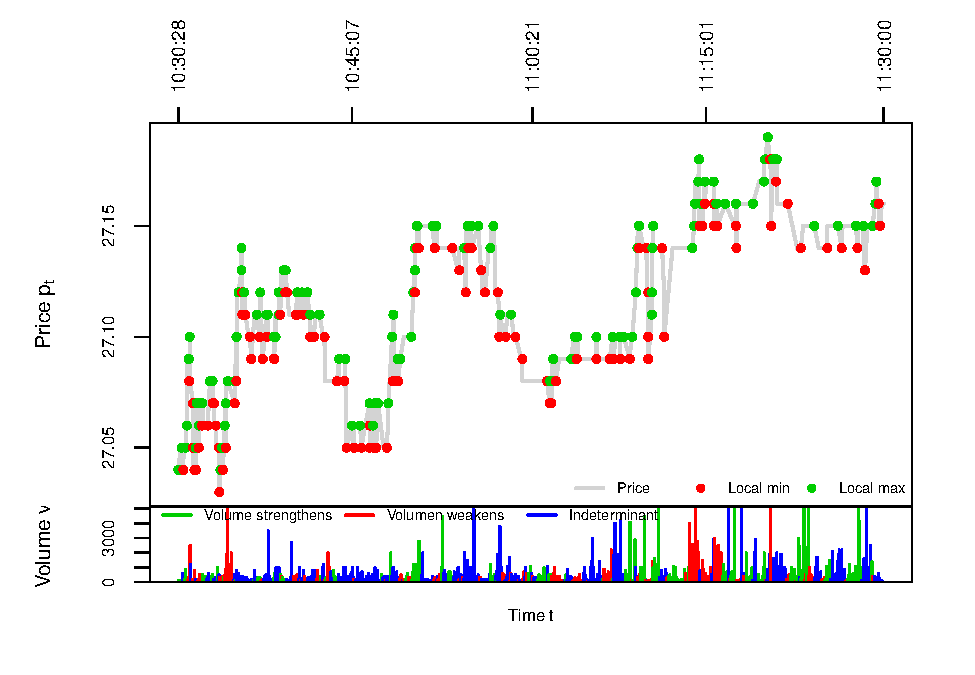
\includegraphics[width=\textwidth]{main_files/figure-latex/unnamed-chunk-7-1} \caption{Local extrema detected in TSE:G 2007-05-11 10:30:00/2007-05-11 11:30:00. \label{tseg-ins-extrema}}\label{fig:unnamed-chunk-7}
\end{figure}

The Features

\begin{verbatim}
## Warning in par(cex.names = 0.7, cex.axis = 0.7, cex.lab = 0.7, cex.main =
## 0.7): "cex.names" is not a graphical parameter
\end{verbatim}

\begin{figure}[H]
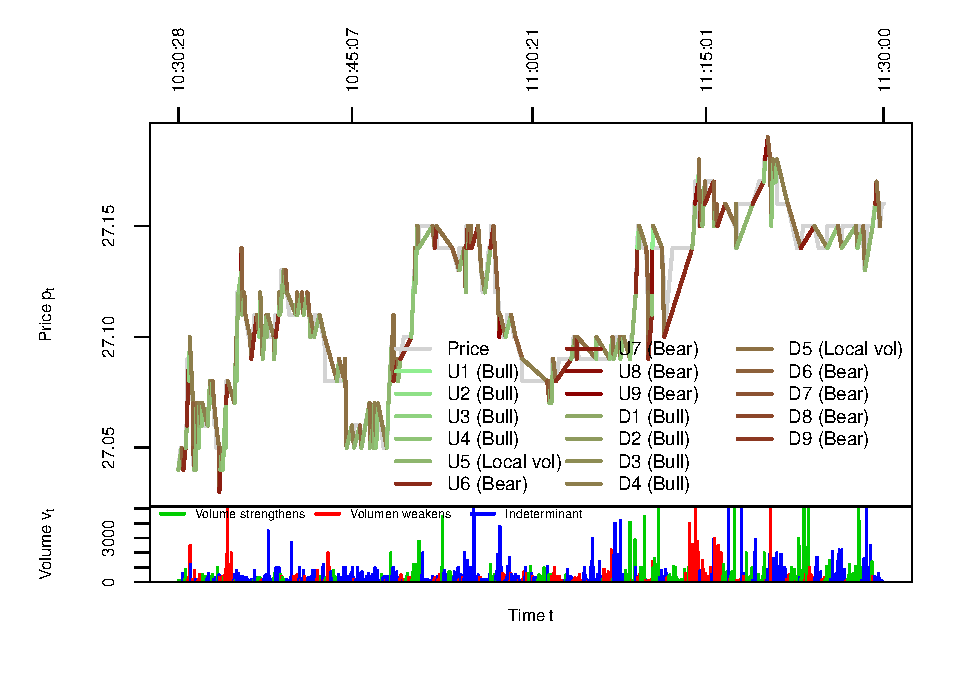
\includegraphics[width=\textwidth]{main_files/figure-latex/unnamed-chunk-8-1} \caption{Features extracted from TSE:G 2007-05-11 10:30:00/2007-05-11 11:30:00. \label{tseg-ins-features}}\label{fig:unnamed-chunk-8}
\end{figure}

\subsubsection{Estimation}\label{estimation}

Model parameters can be segregated into two groups: parameters for the
hidden model, including the initial distribution vector as well as the
transition matrix, and parameters for the conditional multinomial
distributions for the output. Table \ref{tab:tseg-ins-transition}
summarises the former. The estimates for the initial distribution
probabilities \(\pi_1\) and \(1 - \pi_1\) are uncertain to a large
extent, which is unsurprising as the sample provides with only one
starting observation and the model imposes almost no prior information
for the parameters. Team (2017), a technical manual for a programming
language that also contains many brief discussion of statistical
notions, describes some alternative specifications. If the sample were
conceived as a subsequence of a long-running data generating process,
the initial probabilities may be set to equal the stationary state
probabilities of the transition Markov chain. Contrarily, if the sample
was considered a finite-length sequence, the model may have a different
starting distribution.

On the other hand, estimation of the transition parameters profit from a
larger number of trades: more information reduce uncertainty. We note
that the bull top state seems persistent as positive zig-zags \(z^2_3\)
are more likely to transition to bull negative zig-zags \(z^2_4\) versus
bear negative zig-zags \(z^2_1\) by a factor of
\(a_{34} / a_{31} \approx 10\). After studying several stocks and
timespans, we decide that these empirical observations are specific to
the sample and are highly influenced by the general price trend present
in the five day-long training dataset.

\begin{verbatim}
## Warning in par(cex.names = 0.7, cex.axis = 0.7, cex.lab = 0.7, cex.main =
## 0.7): "cex.names" is not a graphical parameter
\end{verbatim}

\begin{table}[ht]
\centering
\begingroup\footnotesize
\begin{tabularx}{0.65 \textwidth}{rRRRRR}
  \toprule
 & Mean & Std. Deviation & $q_{10\%}$ & $q_{50\%}$ & $q_{90\%}$ \\ 
  \midrule
$\pi_{1}$ & 0.51 & 0.28 & 0.10 & 0.52 & 0.89 \\ 
  $1 - \pi_{1}$ & 0.49 & 0.28 & 0.11 & 0.48 & 0.90 \\ 
  $a_{12}$ & 0.46 & 0.11 & 0.31 & 0.47 & 0.58 \\ 
  $1 - a_{12}$ & 0.54 & 0.11 & 0.42 & 0.53 & 0.69 \\ 
  $a_{21}$ & 1.00 & 0.00 & 1.00 & 1.00 & 1.00 \\ 
  $a_{31}$ & 0.09 & 0.06 & 0.02 & 0.08 & 0.17 \\ 
  $1 - a_{31}$ & 0.91 & 0.06 & 0.83 & 0.92 & 0.98 \\ 
  $a_{43}$ & 1.00 & 0.00 & 1.00 & 1.00 & 1.00 \\ 
   \bottomrule
\end{tabularx}
\endgroup
\caption{Estimated parameters of the transition matrix 
               for TSE:G 2007-05-04 09:30:00/2007-05-10 16:30:00.} 
\label{tab:tseg-ins-transition}
\end{table}

Output distributions are summarized in Figure
\textbackslash{}ref\{fig:tseg-ins-multinomial\}. It is important to note
that zig-zags with no price trends \(D_4, D_5, D_6, U_4, U_5, U_6\) are
the most preeminent features. In particular, it is worthwhile to analyse
the behaviour of the model in the presence of local volatility
\(D_5, U_5\), i.e.~when there is no clear trends in price and volume.

\begin{verbatim}
## Warning in par(cex.names = 0.7, cex.axis = 0.7, cex.lab = 0.7, cex.main =
## 0.7): "cex.names" is not a graphical parameter
\end{verbatim}

\begin{figure}[H]
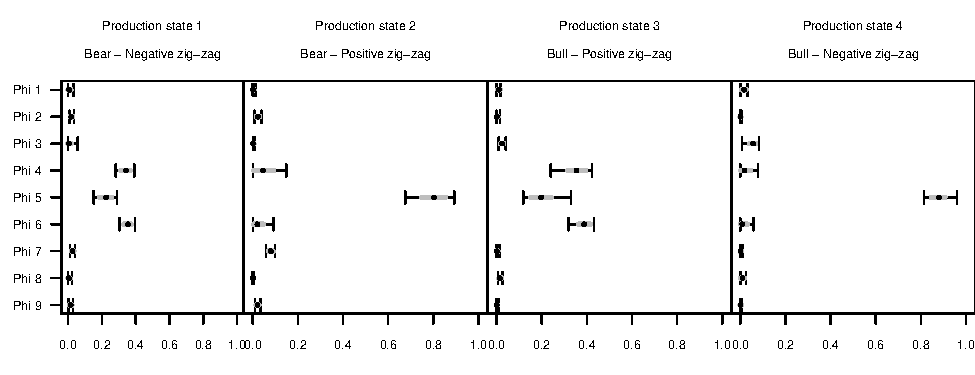
\includegraphics[width=\textwidth]{main_files/figure-latex/unnamed-chunk-11-1} \caption{Estimated parameters of the conditional multinomial distribution of the outputs given the emission state (bottom node) for TSE:G 2007-05-04 09:30:00/2007-05-10 16:30:00. \label{fig:tseg-ins-multinomial}}\label{fig:unnamed-chunk-11}
\end{figure}

We first study short-term price changes in the opposite direction to the
long-term trend. The vast majority of negative zig-zags observed in
bullish markets are due to local volatility (\(\hat{\phi}_{45}\) = 0.88)
as do most of the positive zig-zags found in bearish markets
(\(\hat{\phi}_{25}\) = 0.80). We note, however, that negative legs with
no price trends but weakening or strengthening trade volume are equally
probable in bearish markets
(\(\hat{\phi}_{14} \approx \hat{\phi}_{16}\)). Analogously, we find in
bullish markets that \(\hat{\phi}_{34} \approx \hat{\phi}_{36}\). These
observations counter the a priori classification stated in Table
\ref{tab:feature-space}.

Additionally, we find that positive zig-zags originated in local
volatility are more likely to be seen in bearish markets versus bullish
markets by a factor of \(\phi_{25} / \phi_{35} \approx 4\). The odds for
negative zig-zags are similar. We warn the reader that the current model
needs more information to classify this feature. All in all, we are
warned that zig-zag direction \(f^0\) and change in volume \(f^2\) are
not decisive without a price trend, a hint that the current model needs
either better feature engineering rules for the change in volume or more
external information to deal with local volatility.

\subsubsection{Convergence}\label{convergence}

Figure \ref{tseg-ins-diags} illustrates the trace plot of some arbitrary
parameters as well as some diagnostic measures. In general terms, mixing
and convergence to the stationary distribution is acceptable. The shrink
factor of (Gelman and Rubin 1992), close to \(1\) for all hidden
quantities, indicates an adequate degree of convergence. Sampling is
efficient as signaled by effective sample size ratios near to \(1\) and
Monte Carlo Standar Error to posterior standard deviation ratios well
below 10\%.

\begin{verbatim}
## Warning in par(cex.names = 0.7, cex.axis = 0.7, cex.lab = 0.7, cex.main =
## 0.7): "cex.names" is not a graphical parameter
\end{verbatim}

\begin{figure}[H]
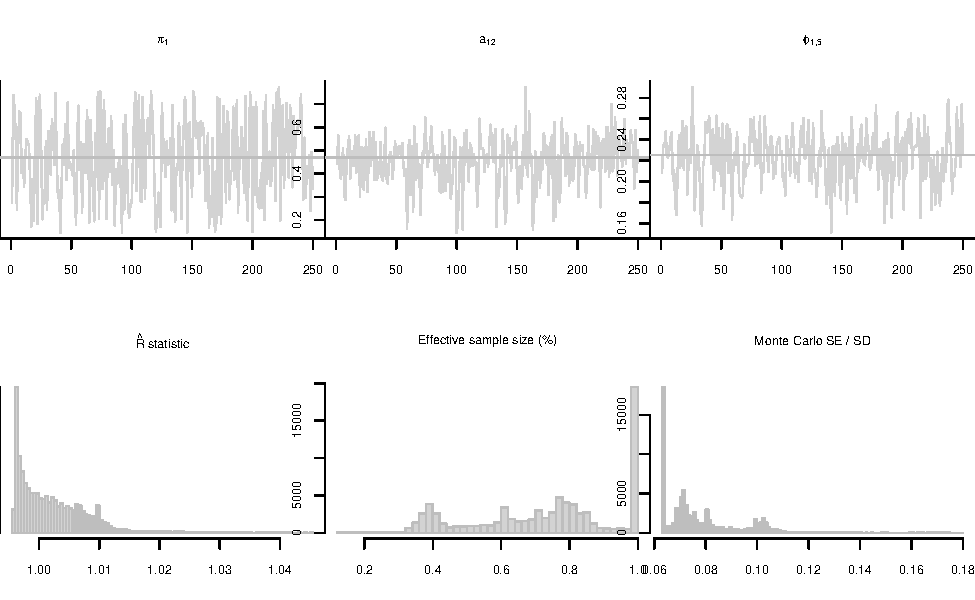
\includegraphics[width=\textwidth]{main_files/figure-latex/unnamed-chunk-12-1} \caption{Traceplot of some arbitrarily selected parameters and histograms of diagnostic measures. Mixing, convergence to the stationary distribution and sampling efficiency are acceptable.\label{tseg-ins-diags}}\label{fig:unnamed-chunk-12}
\end{figure}

Although re-estating the original Hierarchical Hidden Markov Model into
a Hidden Markov Model may increase time and memory complexity, the new
model becomes significantly easier to program and convergence. A full
list of our results, including convergence statistics such as
\(\hat{R}\) and the effective sample size, is included in the Appendix
Section \ref{sec:appendix-tseg-parameters}.

\subsubsection{State probability}\label{state-probability}

\begin{verbatim}
## [1] "% BEFORE AN EVENTUAL SWITCH: \n              bottom nodes 1, 2 (bear) have a mean return of -0.0090%, \n              while bottom nodes 3, 4 (bull) have a mean return of 0.0051%."
\end{verbatim}

The forward algorithm allows us to calculate the filtered belief state:
the probability that an observation at time \(t\) was emitted by one of
the possible four states (bottom-nodes) given the evidence avaliable up
to \(t\). We assign each observation to the emission state with largest
filtered probability and, by the definition of the hierarchical model,
they become naturally linked to one of the two possible top states
(bears and bulls). Figure \ref{tseg-ins-features-hist} reflects the
resulting classification.

\begin{verbatim}
## Warning in par(cex.names = 0.7, cex.axis = 0.7, cex.lab = 0.7, cex.main =
## 0.7): "cex.names" is not a graphical parameter
\end{verbatim}

\begin{figure}[H]
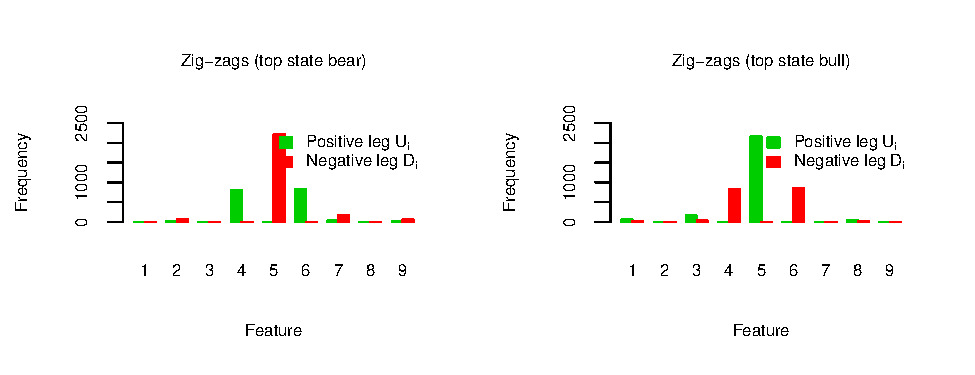
\includegraphics[width=\textwidth]{main_files/figure-latex/unnamed-chunk-14-1} \caption{Distribution of features conditional on the estimated hidden regime (top node). \label{tseg-ins-features-hist}}\label{fig:unnamed-chunk-14}
\end{figure}

The following table provides some summary statistics for the returns of
the observations classified in each state. The structure of the top
nodes are symmetrical and they do not have an a priori order. We label
them according to the in-sample mean trade returns.

\begin{verbatim}
## Warning in par(cex.names = 0.7, cex.axis = 0.7, cex.lab = 0.7, cex.main =
## 0.7): "cex.names" is not a graphical parameter
\end{verbatim}

\begin{table}[ht]
\centering
\begingroup\footnotesize
\begin{tabularx}{\textwidth}{rRRRRRRRRR}
  \toprule
 & Mean & SD & Skewness & Kurtosis & $q_{25}\%$ & $q_{50}\%$ & $q_{75}\%$ & Mean length & Median length \\ 
  \midrule
Bear & -0.01 & 0.06 & 7.97 & 237.46 & -0.04 & 0.00 & 0.00 & 10.62 & 6.00 \\ 
  Bull & 0.00 & 0.05 & 0.97 & 9.37 & 0.00 & 0.00 & 0.04 & 10.17 & 6.00 \\ 
  Unconditional & -0.00 & 0.06 & 5.53 & 173.81 & -0.04 & 0.00 & 0.00 & 10.40 & 6.00 \\ 
   \bottomrule
\end{tabularx}
\endgroup
\caption{Summary statistics for the return of the trades 
               assigned to each of the two possible top states for 
               TSE:G 2007-05-04 09:30:00/2007-05-10 16:30:00. Trade returns 
               are computed as defined in Section \ref{sec:methodology}. 
               Trade length is computed as the number of ticks involved.
               Returns expressed in percentage. SD means Standard Deviation.} 
\label{tab:tseg-ins-topstate}
\end{table}

Bear and bull top states have negative and positive mean respectively by
construction. As it is also visible in Figure
\ref{fig:tseg-ins-ret-hist}, a positive skewness coefficient for all
states indicates that negative returns tend to overweight positive
returns for this specific stock during the five day long in-sample
dataset. However, bear markets have a marked skew towards negative
returns, becomes more risky in term of extreme events (kurtosis) and
trades in bear markets tend to last one tick more than bulls.

\begin{verbatim}
## Warning in par(cex.names = 0.7, cex.axis = 0.7, cex.lab = 0.7, cex.main =
## 0.7): "cex.names" is not a graphical parameter
\end{verbatim}

\begin{figure}[H]
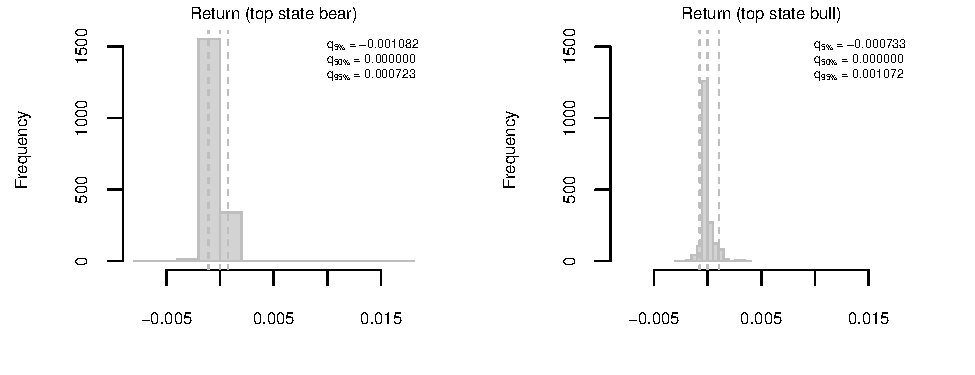
\includegraphics[width=\textwidth]{main_files/figure-latex/unnamed-chunk-16-1} \caption{Conditional distribution of trade returns given the estimated top state in TSE:G 2007-05-04 09:30:00/2007-05-10 16:30:00. \label{fig:tseg-ins-ret-hist}}\label{fig:unnamed-chunk-16}
\end{figure}

We remark that trade returns originated in different stocks or timespans
do not necessarily share these characteristics. Location, dispersion,
symmetry and shape of the return distribution vary along stocks and day
of analysis.

\subsubsection{Fitted output}\label{fitted-output}

As mentioned in Section \ref{sec:model}, the model assumes that outputs
are emitted by one of four possible bottom nodes. By definition,
negative legs belong to either \(z_{1}^2\) or \(z_{4}^2\) while positive
legs belong to \(z_{2}^2\) or \(z_{3}^2\). Once the parameters are
estimated, states \(z_{1}^2\) and \(z_{2}^2\) are labeled as bears while
\(z_{3}^2\) and \(z_{4}^2\) are marked as bulls according to the mean
trade return of the observations belonging to each top node.

Bullish states allow for negative zig-zags and bearish states allow for
positive zig-zags as long as the trade volume is indeterminant or weak.
The results of the classification are summarized in Table
\ref{tab:tseg-filtered-ins}. As expected, the bullish top-node capture
positive movements due to local volatility as well as downward movements
with weak volume.

\subsubsection{\texorpdfstring{We remark that each of the 18 possible
features into one state. For example, observations from feature 3 (ie
U3) are all mapped into state 4. In a sense, this adds very little
information since imputation is almost deterministic once the parameters
are estimated. This is possibly a weakness in the model. See the plot in
\ref{fig:tseg-ins-seqv}.}{We remark that each of the 18 possible features into one state. For example, observations from feature 3 (ie U3) are all mapped into state 4. In a sense, this adds very little information since imputation is almost deterministic once the parameters are estimated. This is possibly a weakness in the model. See the plot in .}}\label{we-remark-that-each-of-the-18-possible-features-into-one-state.-for-example-observations-from-feature-3-ie-u3-are-all-mapped-into-state-4.-in-a-sense-this-adds-very-little-information-since-imputation-is-almost-deterministic-once-the-parameters-are-estimated.-this-is-possibly-a-weakness-in-the-model.-see-the-plot-in-.}

\begin{verbatim}
## Warning in par(cex.names = 0.7, cex.axis = 0.7, cex.lab = 0.7, cex.main =
## 0.7): "cex.names" is not a graphical parameter
\end{verbatim}

\begin{table}[ht]
\centering
\begingroup\scriptsize
\begin{tabularx}{\textwidth}{rRRRRRRRRRRRRRRRRRRR}
  \toprule
Top & Bottom & $U_{1}$ & $U_{2}$ & $U_{3}$ & $U_{4}$ & $U_{5}$ & $U_{6}$ & $U_{7}$ & $U_{8}$ & $U_{9}$ & $D_{1}$ & $D_{2}$ & $D_{3}$ & $D_{4}$ & $D_{5}$ & $D_{6}$ & $D_{7}$ & $D_{8}$ & $D_{9}$ \\ 
  \midrule
Bear & 1 & 0 & 15 & 0 & 810 & 0 & 828 & 33 & 0 & 17 & 0 & 0 & 0 & 0 & 0 & 0 & 0 & 0 & 0 \\ 
  Bear & 2 & 0 & 0 & 0 & 0 & 0 & 0 & 0 & 0 & 0 & 0 & 72 & 0 & 0 & 2208 & 0 & 181 & 0 & 59 \\ 
  Bull & 3 & 0 & 0 & 0 & 0 & 0 & 0 & 0 & 27 & 0 & 15 & 0 & 34 & 831 & 0 & 846 & 0 & 16 & 0 \\ 
  Bull & 4 & 58 & 0 & 158 & 0 & 2155 & 0 & 0 & 22 & 0 & 0 & 0 & 0 & 0 & 1 & 0 & 0 & 0 & 0 \\ 
   \bottomrule
\end{tabularx}
\endgroup
\caption{Features extracted are classified as emitted by one
               of the four possible bottom-nodes according to the filtered
               probability. TSE:G 2007-05-04 09:30:00/2007-05-10 16:30:00.} 
\label{tab:tseg-filtered-ins}
\end{table}

Now, look how at how the features are classified: Mention plot number on
tayal.

\begin{verbatim}
## Warning in par(cex.names = 0.7, cex.axis = 0.7, cex.lab = 0.7, cex.main =
## 0.7): "cex.names" is not a graphical parameter
\end{verbatim}

\begin{figure}[H]
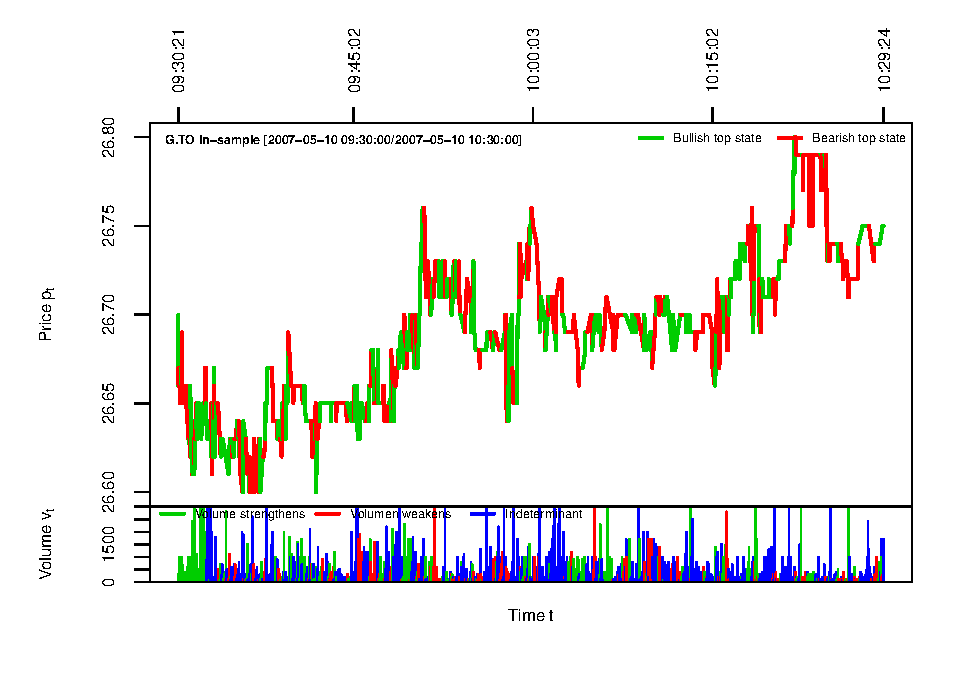
\includegraphics[width=\textwidth]{main_files/figure-latex/unnamed-chunk-18-1} \caption{Tick by tick sequence of trades, classified as belonging to the bear or the bull top state, from TSE:G 2007-05-10 09:30:00/2007-05-10 10:30:00. \label{fig:tseg-ins-seqv}}\label{fig:unnamed-chunk-18}
\end{figure}

\subsubsection{Trading Strategy}\label{trading-strategy}

Using the parameters estimated from the five days of training data, we
run the trading strategy out of sample during one day.

\paragraph{After a zig-zag leg is completed, the trading system buys one
unit every time the top-level state switches to bullish (a run) and
sells one unit every time it switches to bearish (a reveral). As an
addition to Tayal (2009), where trades are executed one tick after the
zig-zag leg is observed to ensure there is no lock-ahead bias, we
investigate the decay of the strategy performance for longer
lags.}\label{after-a-zig-zag-leg-is-completed-the-trading-system-buys-one-unit-every-time-the-top-level-state-switches-to-bullish-a-run-and-sells-one-unit-every-time-it-switches-to-bearish-a-reveral.-as-an-addition-to-tayal2009regime-where-trades-are-executed-one-tick-after-the-zig-zag-leg-is-observed-to-ensure-there-is-no-lock-ahead-bias-we-investigate-the-decay-of-the-strategy-performance-for-longer-lags.}

\blandscape
\newpage

\begin{figure}[H]
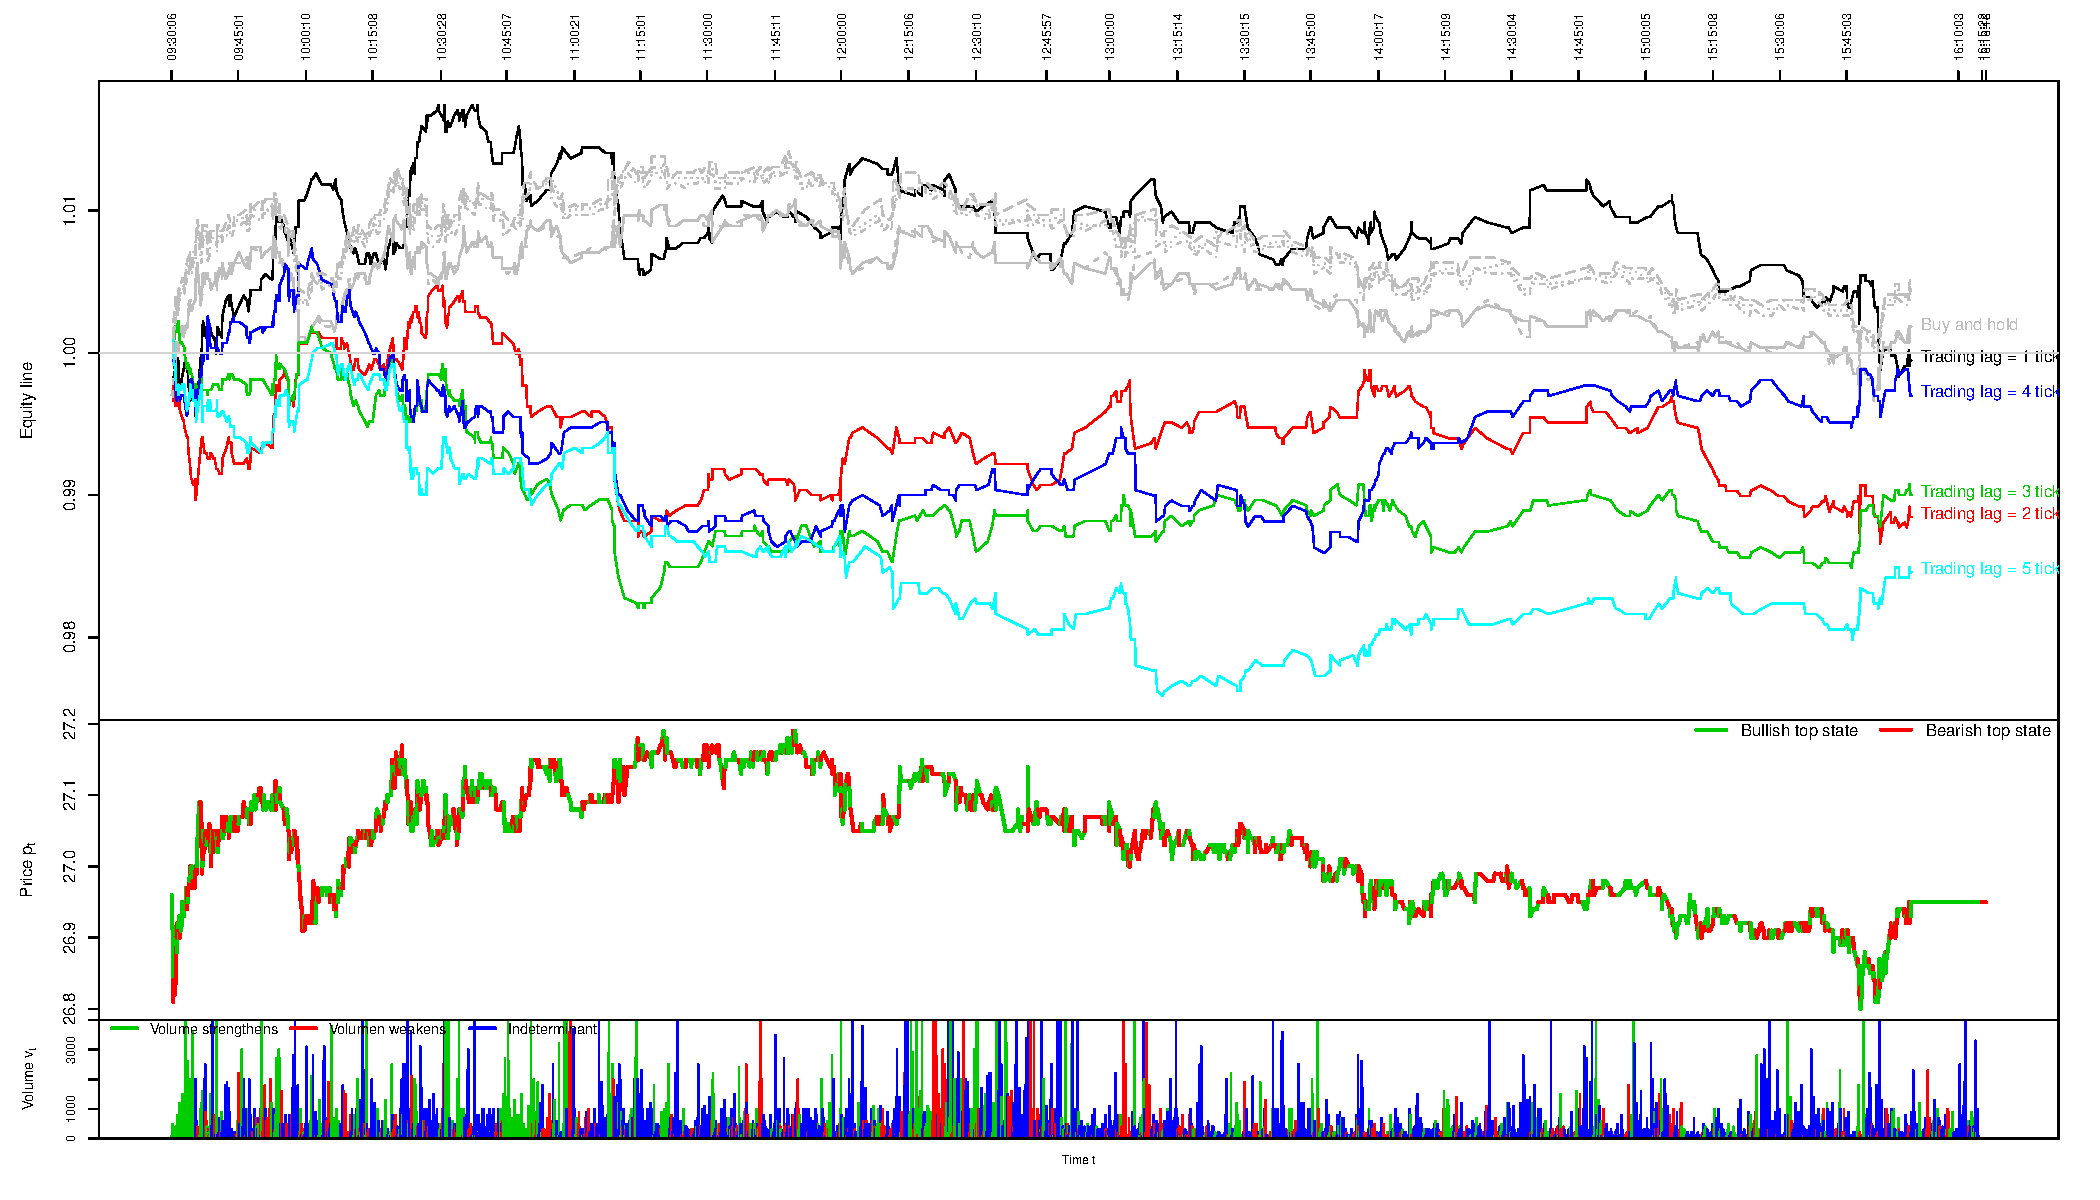
\includegraphics[width=1\linewidth]{main_files/figure-latex/unnamed-chunk-19-1} \caption{Tick by tick sequence of trades, classified as belonging to the bear or the bull top state, from TSE:G 2007-05-10 09:30:00/2007-05-10 10:30:00. \label{fig:tseg-ins-seqv}}\label{fig:unnamed-chunk-19}
\end{figure}

\elandscape

\paragraph{Walking forward backtest}\label{walking-forward-backtest}

\begin{verbatim}
## Warning in par(cex.names = 0.7, cex.axis = 0.7, cex.lab = 0.7, cex.main =
## 0.7): "cex.names" is not a graphical parameter
\end{verbatim}

\begin{table}[ht]
\centering
\begingroup\scriptsize
\begin{tabularx}{\textwidth}{rRRRRRRR}
  \toprule
 & Buy-Hold & HHMM (0 lag) & HHMM (1 lag) & HHMM (2 lag) & HHMM (3 lag) & HHMM (4 lag) & HHMM (5 lag) \\ 
  \midrule
2007-05-08 & -0.01 & 0.04 & -0.02 & -0.01 & 0.01 & 0.01 & 0.02 \\ 
  2007-05-09 & -0.00 & 0.04 & 0.00 & 0.02 & 0.02 & 0.01 & 0.01 \\ 
  2007-05-10 & -0.00 & 0.04 & 0.01 & -0.01 & 0.02 & 0.02 & 0.00 \\ 
  2007-05-11 & -0.00 & 0.00 & 0.00 & 0.01 & -0.00 & -0.01 & 0.00 \\ 
  2007-05-14 & -0.03 & 0.03 & -0.01 & 0.01 & -0.01 & -0.00 & -0.01 \\ 
  2007-05-15 & -0.00 & 0.03 & -0.00 & 0.00 & 0.02 & 0.02 & 0.00 \\ 
  2007-05-16 & -0.00 & 0.05 & -0.01 & -0.00 & 0.01 & 0.03 & -0.02 \\ 
  2007-05-17 & -0.00 & -0.02 & 0.00 & 0.02 & 0.00 & -0.03 & -0.00 \\ 
  2007-05-18 & 0.01 & -0.01 & 0.01 & 0.00 & 0.02 & 0.01 & 0.02 \\ 
  2007-05-22 & -0.02 & -0.02 & -0.02 & 0.02 & 0.01 & 0.02 & 0.02 \\ 
  2007-05-23 & -0.01 & 0.02 & -0.00 & -0.01 & -0.01 & 0.01 & 0.01 \\ 
  2007-05-24 & -0.03 & 0.02 & -0.00 & -0.01 & -0.01 & -0.00 & -0.02 \\ 
  2007-05-25 & 0.00 & -0.01 & -0.01 & 0.00 & 0.01 & -0.02 & -0.02 \\ 
  2007-05-28 & -0.01 & -0.02 & -0.01 & 0.01 & -0.01 & -0.01 & 0.02 \\ 
  2007-05-29 & -0.02 & -0.02 & -0.01 & -0.02 & -0.00 & 0.02 & 0.01 \\ 
  2007-05-30 & 0.01 & -0.02 & -0.03 & -0.03 & -0.01 & -0.04 & -0.02 \\ 
  2007-05-31 & 0.04 & 0.00 & -0.01 & -0.01 & -0.02 & -0.01 & -0.03 \\ 
   \midrule
Total & -0.09 & 0.17 & -0.12 & -0.01 & 0.04 & 0.02 & -0.02 \\ 
   \bottomrule
\end{tabularx}
\endgroup
\caption{Compound daily return originated in the HHMM trading strategy for different levels of lags. Returns from the buy and hold strategy are included as a reference. Returns expressed in percentage. Lag measured in ticks between the end of the zig-zag and the execution of the trade (zero lag suffers from look-ahead bias). TSE:G.} 
\label{tab:tseg-filtered-ins}
\end{table}

\ldots{}

\subsubsection{Trading strategy}\label{trading-strategy-1}

Show total for other stocks and mention strat vs bh.

\ldots{}

\subsection{Discussion}\label{further-research}

\subsubsection{The statistical model}\label{the-statistical-model}

We find that the model proposed, while statistically simple, is highly
expressive of financial domain knowledge. The hierarchical design
creates a multi-level stochastic process that learns autocorrelations in
different time scales. This accommodates for multiresolution, a typical
characterstic of financial datasets. We remark that, whereas HHMM offer
a methodology to create a complex, highly non linear model for time
series, estimation and inference can be achieved in reasonable
complexity. The developments by Murphy and Paskin (2001) simplified
cubic time into linear time inference, making inference feasible for
high-frequency finance.

\subsubsection{The financial
application}\label{the-financial-application}

We have special interest in the feature extraction procedure. They were
cleverly designed to reproduce some of the most basic principles of
technical analysis and, when applied to real data, they proved to be a
powerful descriptor of price and volume movements. Nonetheless, we
observe that the change in volume is the weakest component and provides
with great opportunities for further enhancements. The contribution of
the author should not be neglected: in general terms, the features are
the most important factor in the success or the failure of a machine
learning project(Domingos 2012).

\begin{center}\rule{0.5\linewidth}{\linethickness}\end{center}

\section{References}\label{references}

\hypertarget{refs}{}
\hypertarget{ref-carpenter2016stan}{}
Carpenter, Bob, Andrew Gelman, Matt Hoffman, Daniel Lee, Ben Goodrich,
Michael Betancourt, Michael A Brubaker, Jiqiang Guo, Peter Li, and Allen
Riddell. 2016. ``Stan: A Probabilistic Programming Language.''
\emph{Journal of Statistical Software} 20.

\hypertarget{ref-domingos2012few}{}
Domingos, Pedro. 2012. ``A Few Useful Things to Know About Machine
Learning.'' \emph{Commun. ACM} 55 (10). New York, NY, USA: ACM: 78--87.
doi:\href{https://doi.org/10.1145/2347736.2347755}{10.1145/2347736.2347755}.

\hypertarget{ref-fine1998hierarchical}{}
Fine, Shai, and Yoram Singer. 1998. ``The Hierarchical Hidden Markov
Model: Analysis and Applications.''

\hypertarget{ref-gelman1992inference}{}
Gelman, Andrew, and Donald B Rubin. 1992. ``Inference from Iterative
Simulation Using Multiple Sequences.'' \emph{Statistical Science}.
JSTOR, 457--72.

\hypertarget{ref-murphy2001linear}{}
Murphy, Kevin P., and Mark A. Paskin. 2001. ``Linear Time Inference in
Hierarchical Hmms.''

\hypertarget{ref-ord2008secret}{}
Ord, Tim. 2008. ``The Secret Science of Price and Volume.'' \emph{Master
Traders: Strategies for Superior Returns from Today's Top Traders}.
Wiley Online Library, 87--105.

\hypertarget{ref-sandoval2015computational}{}
Sandoval, Javier, and Germán Hernández. 2015. ``Computational Visual
Analysis of the Order Book Dynamics for Creating High-Frequency Foreign
Exchange Trading Strategies.'' \emph{Procedia Computer Science} 51.
Elsevier: 1593--1602.

\hypertarget{ref-tayal2009regime}{}
Tayal, Aditya. 2009. ``Regime Switching and Technical Trading with
Dynamic Bayesian Networks in High-Frequency Stock Markets.''
Master's thesis, University of Waterloo.

\hypertarget{ref-team2017stan}{}
Team, Stan Development. 2017. \emph{Stan Modeling Language: User's Guide
and Reference Manual: Version 2.15.0.}

\hypertarget{ref-wisebourt2011hierarchical}{}
Wisebourt, Shaul Sergey. 2011. ``Hierarchical Hidden Markov Model of
High-Frequency Market Regimes Using Trade Price and Limit Order Book
Information.'' Master's thesis, University of Waterloo.

\begin{center}\rule{0.5\linewidth}{\linethickness}\end{center}

\section{Appendix}\label{appendix}

\subsection{Estimated parameters TSE:G
2007-05-04/2007-05-10.}\label{estimated-parameters-tseg-2007-05-042007-05-10.}

\label{sec:appendix-tseg-parameters}

\begin{verbatim}
## Warning in par(cex.names = 0.7, cex.axis = 0.7, cex.lab = 0.7, cex.main =
## 0.7): "cex.names" is not a graphical parameter
\end{verbatim}

\begin{table}[ht]
\centering
\begingroup\footnotesize
\begin{tabularx}{\textwidth}{lRRRRRRRRRRRR}
  \toprule
 & Mean & MCSE & SD & $q_{2.5\%}$ & $q_{10.0\%}$ & $q_{25.0\%}$ & $q_{50.0\%}$ & $q_{75.0\%}$ & $q_{90.0\%}$ & $q_{97.5\%}$ & ESS & $\hat{R}$ \\ 
  \midrule
$\pi_{1}$ & 0.51 & 0.02 & 0.28 & 0.03 & 0.10 & 0.27 & 0.52 & 0.74 & 0.89 & 0.96 & 250.00 & 1.00 \\ 
  $\pi_{2}$ & 0.00 & 0.00 & 0.00 & 0.00 & 0.00 & 0.00 & 0.00 & 0.00 & 0.00 & 0.00 & 250.00 & n.a. \\ 
  $\pi_{3}$ & 0.49 & 0.02 & 0.28 & 0.04 & 0.11 & 0.26 & 0.48 & 0.73 & 0.90 & 0.97 & 250.00 & 1.00 \\ 
  $\pi_{4}$ & 0.00 & 0.00 & 0.00 & 0.00 & 0.00 & 0.00 & 0.00 & 0.00 & 0.00 & 0.00 & 250.00 & n.a. \\ 
   \midrule
$a_{11}$ & 0.00 & 0.00 & 0.00 & 0.00 & 0.00 & 0.00 & 0.00 & 0.00 & 0.00 & 0.00 & 250.00 & n.a. \\ 
  $a_{12}$ & 0.46 & 0.01 & 0.11 & 0.19 & 0.31 & 0.39 & 0.47 & 0.53 & 0.58 & 0.64 & 119.70 & 1.00 \\ 
  $a_{13}$ & 0.54 & 0.01 & 0.11 & 0.36 & 0.42 & 0.47 & 0.53 & 0.61 & 0.69 & 0.81 & 119.70 & 1.00 \\ 
  $a_{14}$ & 0.00 & 0.00 & 0.00 & 0.00 & 0.00 & 0.00 & 0.00 & 0.00 & 0.00 & 0.00 & 250.00 & n.a. \\ 
  $a_{21}$ & 1.00 & 0.00 & 0.00 & 1.00 & 1.00 & 1.00 & 1.00 & 1.00 & 1.00 & 1.00 & 250.00 & n.a. \\ 
  $a_{22}$ & 0.00 & 0.00 & 0.00 & 0.00 & 0.00 & 0.00 & 0.00 & 0.00 & 0.00 & 0.00 & 250.00 & n.a. \\ 
  $a_{23}$ & 0.00 & 0.00 & 0.00 & 0.00 & 0.00 & 0.00 & 0.00 & 0.00 & 0.00 & 0.00 & 250.00 & n.a. \\ 
  $a_{24}$ & 0.00 & 0.00 & 0.00 & 0.00 & 0.00 & 0.00 & 0.00 & 0.00 & 0.00 & 0.00 & 250.00 & n.a. \\ 
  $a_{31}$ & 0.09 & 0.00 & 0.06 & 0.00 & 0.02 & 0.04 & 0.08 & 0.13 & 0.17 & 0.24 & 198.87 & 1.00 \\ 
  $a_{32}$ & 0.00 & 0.00 & 0.00 & 0.00 & 0.00 & 0.00 & 0.00 & 0.00 & 0.00 & 0.00 & 250.00 & n.a. \\ 
  $a_{33}$ & 0.00 & 0.00 & 0.00 & 0.00 & 0.00 & 0.00 & 0.00 & 0.00 & 0.00 & 0.00 & 250.00 & n.a. \\ 
  $a_{34}$ & 0.91 & 0.00 & 0.06 & 0.76 & 0.83 & 0.87 & 0.92 & 0.96 & 0.98 & 1.00 & 198.87 & 1.00 \\ 
  $a_{41}$ & 0.00 & 0.00 & 0.00 & 0.00 & 0.00 & 0.00 & 0.00 & 0.00 & 0.00 & 0.00 & 250.00 & n.a. \\ 
  $a_{42}$ & 0.00 & 0.00 & 0.00 & 0.00 & 0.00 & 0.00 & 0.00 & 0.00 & 0.00 & 0.00 & 250.00 & n.a. \\ 
  $a_{43}$ & 1.00 & 0.00 & 0.00 & 1.00 & 1.00 & 1.00 & 1.00 & 1.00 & 1.00 & 1.00 & 250.00 & n.a. \\ 
  $a_{44}$ & 0.00 & 0.00 & 0.00 & 0.00 & 0.00 & 0.00 & 0.00 & 0.00 & 0.00 & 0.00 & 250.00 & n.a. \\ 
   \midrule
$\phi_{11}$ & 0.01 & 0.00 & 0.01 & 0.00 & 0.00 & 0.00 & 0.01 & 0.01 & 0.02 & 0.02 & 99.42 & 1.01 \\ 
  $\phi_{12}$ & 0.02 & 0.00 & 0.00 & 0.01 & 0.01 & 0.02 & 0.02 & 0.02 & 0.03 & 0.03 & 250.00 & 1.00 \\ 
  $\phi_{13}$ & 0.01 & 0.00 & 0.01 & 0.00 & 0.00 & 0.00 & 0.00 & 0.01 & 0.02 & 0.03 & 102.05 & 1.02 \\ 
  $\phi_{14}$ & 0.34 & 0.00 & 0.02 & 0.29 & 0.31 & 0.33 & 0.34 & 0.36 & 0.37 & 0.38 & 150.07 & 1.01 \\ 
  $\phi_{15}$ & 0.22 & 0.00 & 0.03 & 0.17 & 0.19 & 0.21 & 0.23 & 0.24 & 0.26 & 0.27 & 171.58 & 1.01 \\ 
  $\phi_{16}$ & 0.35 & 0.00 & 0.02 & 0.31 & 0.33 & 0.34 & 0.35 & 0.37 & 0.37 & 0.39 & 250.00 & 1.00 \\ 
  $\phi_{17}$ & 0.03 & 0.00 & 0.01 & 0.02 & 0.02 & 0.02 & 0.03 & 0.03 & 0.03 & 0.04 & 250.00 & 1.00 \\ 
  $\phi_{18}$ & 0.01 & 0.00 & 0.00 & 0.00 & 0.00 & 0.00 & 0.00 & 0.01 & 0.01 & 0.02 & 144.00 & 1.00 \\ 
  $\phi_{19}$ & 0.02 & 0.00 & 0.00 & 0.01 & 0.01 & 0.01 & 0.02 & 0.02 & 0.02 & 0.03 & 250.00 & 1.00 \\ 
  $\phi_{21}$ & 0.00 & 0.00 & 0.00 & 0.00 & 0.00 & 0.00 & 0.00 & 0.00 & 0.00 & 0.01 & 66.44 & 1.01 \\ 
  $\phi_{22}$ & 0.02 & 0.00 & 0.01 & 0.01 & 0.02 & 0.02 & 0.02 & 0.03 & 0.03 & 0.03 & 250.00 & 1.00 \\ 
  $\phi_{23}$ & 0.00 & 0.00 & 0.00 & 0.00 & 0.00 & 0.00 & 0.00 & 0.00 & 0.00 & 0.01 & 250.00 & 1.00 \\ 
  $\phi_{24}$ & 0.05 & 0.00 & 0.03 & 0.00 & 0.01 & 0.02 & 0.05 & 0.07 & 0.09 & 0.12 & 102.30 & 1.00 \\ 
  $\phi_{25}$ & 0.80 & 0.00 & 0.04 & 0.72 & 0.75 & 0.78 & 0.80 & 0.83 & 0.85 & 0.87 & 90.82 & 1.00 \\ 
  $\phi_{26}$ & 0.02 & 0.00 & 0.02 & 0.00 & 0.00 & 0.01 & 0.02 & 0.03 & 0.05 & 0.07 & 194.25 & 1.00 \\ 
  $\phi_{27}$ & 0.08 & 0.00 & 0.01 & 0.06 & 0.07 & 0.07 & 0.08 & 0.09 & 0.09 & 0.10 & 250.00 & 1.00 \\ 
  $\phi_{28}$ & 0.00 & 0.00 & 0.00 & 0.00 & 0.00 & 0.00 & 0.00 & 0.00 & 0.00 & 0.00 & 250.00 & 1.00 \\ 
  $\phi_{29}$ & 0.02 & 0.00 & 0.00 & 0.01 & 0.02 & 0.02 & 0.02 & 0.02 & 0.03 & 0.03 & 250.00 & 1.00 \\ 
  $\phi_{31}$ & 0.01 & 0.00 & 0.00 & 0.00 & 0.01 & 0.01 & 0.01 & 0.01 & 0.02 & 0.02 & 52.96 & 1.00 \\ 
  $\phi_{32}$ & 0.00 & 0.00 & 0.00 & 0.00 & 0.00 & 0.00 & 0.00 & 0.00 & 0.01 & 0.01 & 250.00 & 1.00 \\ 
  $\phi_{33}$ & 0.03 & 0.00 & 0.01 & 0.02 & 0.02 & 0.02 & 0.03 & 0.03 & 0.03 & 0.04 & 250.00 & 1.00 \\ 
  $\phi_{34}$ & 0.36 & 0.00 & 0.03 & 0.30 & 0.32 & 0.33 & 0.35 & 0.38 & 0.39 & 0.41 & 111.49 & 1.00 \\ 
  $\phi_{35}$ & 0.20 & 0.00 & 0.04 & 0.14 & 0.15 & 0.17 & 0.20 & 0.22 & 0.24 & 0.28 & 99.99 & 1.00 \\ 
  $\phi_{36}$ & 0.39 & 0.00 & 0.02 & 0.35 & 0.36 & 0.38 & 0.39 & 0.40 & 0.42 & 0.43 & 227.14 & 1.00 \\ 
  $\phi_{37}$ & 0.00 & 0.00 & 0.00 & 0.00 & 0.00 & 0.00 & 0.00 & 0.00 & 0.01 & 0.01 & 250.00 & 1.00 \\ 
  $\phi_{38}$ & 0.02 & 0.00 & 0.00 & 0.01 & 0.01 & 0.01 & 0.02 & 0.02 & 0.02 & 0.02 & 250.00 & 1.00 \\ 
  $\phi_{39}$ & 0.00 & 0.00 & 0.00 & 0.00 & 0.00 & 0.00 & 0.00 & 0.00 & 0.00 & 0.01 & 250.00 & 1.00 \\ 
  $\phi_{41}$ & 0.02 & 0.00 & 0.01 & 0.00 & 0.01 & 0.01 & 0.02 & 0.02 & 0.03 & 0.03 & 75.13 & 1.00 \\ 
  $\phi_{42}$ & 0.00 & 0.00 & 0.00 & 0.00 & 0.00 & 0.00 & 0.00 & 0.00 & 0.00 & 0.00 & 250.00 & 1.00 \\ 
  $\phi_{43}$ & 0.06 & 0.00 & 0.01 & 0.03 & 0.04 & 0.05 & 0.06 & 0.06 & 0.07 & 0.07 & 124.34 & 1.02 \\ 
  $\phi_{44}$ & 0.02 & 0.00 & 0.02 & 0.00 & 0.00 & 0.01 & 0.02 & 0.03 & 0.05 & 0.06 & 178.86 & 1.01 \\ 
  $\phi_{45}$ & 0.88 & 0.00 & 0.02 & 0.83 & 0.85 & 0.86 & 0.88 & 0.90 & 0.91 & 0.93 & 110.86 & 1.02 \\ 
  $\phi_{46}$ & 0.01 & 0.00 & 0.01 & 0.00 & 0.00 & 0.00 & 0.01 & 0.02 & 0.03 & 0.04 & 151.90 & 1.00 \\ 
  $\phi_{47}$ & 0.00 & 0.00 & 0.00 & 0.00 & 0.00 & 0.00 & 0.00 & 0.00 & 0.00 & 0.01 & 250.00 & 1.00 \\ 
  $\phi_{48}$ & 0.01 & 0.00 & 0.01 & 0.00 & 0.00 & 0.01 & 0.01 & 0.01 & 0.02 & 0.02 & 110.72 & 1.00 \\ 
  $\phi_{49}$ & 0.00 & 0.00 & 0.00 & 0.00 & 0.00 & 0.00 & 0.00 & 0.00 & 0.00 & 0.01 & 250.00 & 1.00 \\ 
   \bottomrule
\multicolumn{12}{l}{}\\
\end{tabularx}
\endgroup
\caption{Statistics summary for the distributions of 
                   estimated parameters for TSE:G 2007-05-04 
                   09:30:00/2007-05-10 16:30:00. MCSE means Monte Carlo 
                   Standard Error, SD means (posteriori) Standard Deviation 
                   and ESS means Effective Sample Size.} 
\label{tab:tseg-ins-appendix-summary}
\end{table}

\newpage

\subsection{Walking forward for all
assets}\label{walking-forward-for-all-assets}

\subsubsection{BBDb.TO}\label{bbdb.to}

\begin{verbatim}
## Warning in par(cex.names = 0.7, cex.axis = 0.7, cex.lab = 0.7, cex.main =
## 0.7): "cex.names" is not a graphical parameter
\end{verbatim}

\begin{table}[h!]
\centering
\begingroup\scriptsize
\begin{tabularx}{\textwidth}{rRRRRRRR}
  \toprule
 & Buy-Hold & HHMM (0 lag) & HHMM (1 lag) & HHMM (2 lag) & HHMM (3 lag) & HHMM (4 lag) & HHMM (5 lag) \\ 
  \midrule
2007-05-08 & -0.01 & -0.06 & -0.05 & -0.02 & -0.00 & -0.02 & -0.04 \\ 
  2007-05-09 & -0.01 & 0.00 & -0.06 & -0.01 & -0.04 & 0.03 & 0.00 \\ 
  2007-05-10 & -0.01 & -0.01 & -0.02 & 0.02 & 0.03 & 0.02 & 0.01 \\ 
  2007-05-11 & 0.02 & -0.05 & -0.05 & -0.03 & 0.01 & -0.01 & -0.00 \\ 
  2007-05-14 & -0.00 & -0.12 & -0.14 & -0.03 & -0.03 & -0.01 & -0.01 \\ 
  2007-05-15 & 0.00 & -0.03 & -0.00 & 0.03 & -0.00 & -0.02 & 0.02 \\ 
  2007-05-16 & 0.01 & -0.04 & -0.15 & -0.07 & 0.01 & 0.01 & 0.03 \\ 
  2007-05-17 & 0.01 & 0.00 & -0.03 & -0.01 & 0.01 & 0.02 & 0.01 \\ 
  2007-05-18 & -0.01 & -0.06 & -0.12 & -0.04 & 0.00 & 0.04 & 0.02 \\ 
  2007-05-22 & -0.01 & -0.05 & -0.09 & -0.06 & -0.05 & -0.01 & 0.01 \\ 
  2007-05-23 & -0.02 & -0.10 & -0.18 & -0.04 & 0.01 & 0.03 & 0.05 \\ 
  2007-05-24 & 0.00 & -0.13 & -0.08 & 0.03 & -0.00 & 0.03 & -0.03 \\ 
  2007-05-25 & 0.01 & -0.16 & -0.10 & -0.06 & -0.04 & -0.06 & 0.05 \\ 
  2007-05-28 & 0.01 & -0.10 & -0.09 & -0.04 & -0.02 & -0.02 & 0.04 \\ 
  2007-05-29 & 0.04 & -0.22 & -0.42 & -0.26 & -0.07 & -0.04 & 0.05 \\ 
  2007-05-30 & 0.01 & -0.11 & -0.21 & -0.11 & -0.04 & 0.02 & 0.04 \\ 
  2007-05-31 & -0.03 & 0.01 & 0.00 & 0.09 & 0.05 & 0.01 & 0.03 \\ 
   \midrule
Total & -0.01 & -0.73 & -0.87 & -0.49 & -0.17 & 0.03 & 0.34 \\ 
   \bottomrule
\end{tabularx}
\endgroup
\caption{Compound daily return originated in the HHMM trading strategy for different levels of lags. Returns from the buy and hold strategy are included as a reference. Returns expressed in percentage. Lag measured in ticks between the end of the zig-zag and the execution of the trade (zero lag suffers from look-ahead bias). BBDb.TO} 
\label{tab:appendix-wf-BBDb.TO}
\end{table}

\begin{verbatim}
## Warning in par(cex.names = 0.7, cex.axis = 0.7, cex.lab = 0.7, cex.main =
## 0.7): "cex.names" is not a graphical parameter
\end{verbatim}

\begin{figure}[H]
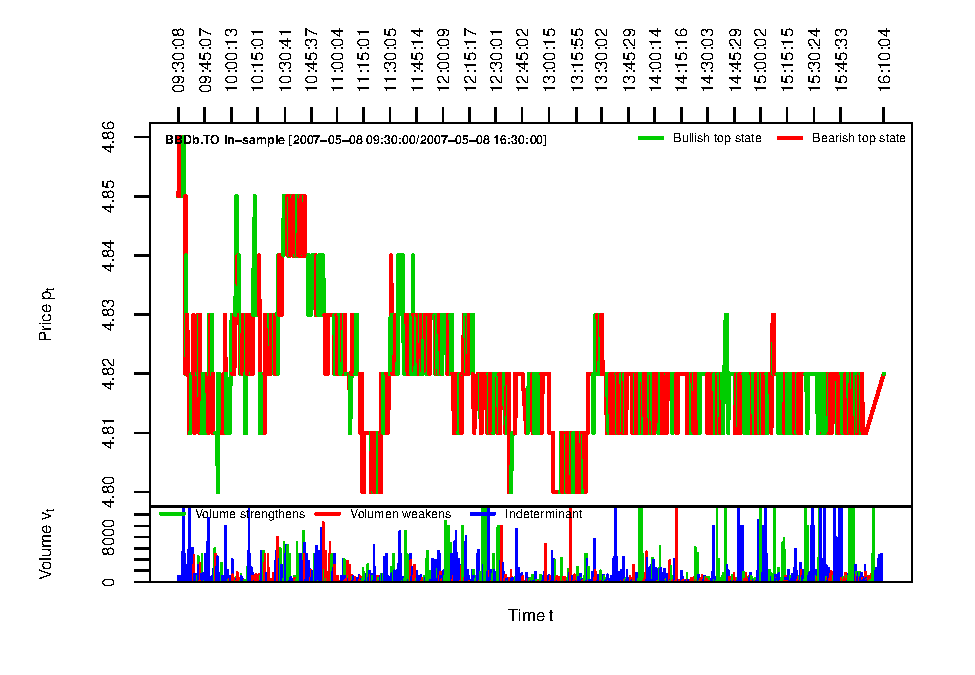
\includegraphics[width=\textwidth]{main_files/figure-latex/unnamed-chunk-26-1} \caption{Tick by tick sequence of trades, classified as belonging to the bear or the bull top state, from `r sym`.}\label{fig:unnamed-chunk-26}
\end{figure}

\newpage

\subsubsection{BCE.TO}\label{bce.to}

\begin{verbatim}
## Warning in par(cex.names = 0.7, cex.axis = 0.7, cex.lab = 0.7, cex.main =
## 0.7): "cex.names" is not a graphical parameter
\end{verbatim}

\begin{table}[h!]
\centering
\begingroup\scriptsize
\begin{tabularx}{\textwidth}{rRRRRRRR}
  \toprule
 & Buy-Hold & HHMM (0 lag) & HHMM (1 lag) & HHMM (2 lag) & HHMM (3 lag) & HHMM (4 lag) & HHMM (5 lag) \\ 
  \midrule
2007-05-08 & 0.01 & -0.02 & 0.02 & 0.00 & -0.02 & 0.01 & 0.01 \\ 
  2007-05-09 & -0.01 & -0.04 & -0.01 & -0.02 & 0.01 & 0.01 & 0.01 \\ 
  2007-05-10 & 0.00 & -0.02 & -0.01 & 0.02 & 0.01 & 0.00 & 0.01 \\ 
  2007-05-11 & -0.00 & 0.00 & -0.01 & 0.01 & -0.01 & -0.01 & -0.01 \\ 
  2007-05-14 & -0.00 & -0.02 & -0.02 & -0.02 & -0.01 & 0.00 & -0.01 \\ 
  2007-05-15 & 0.00 & -0.02 & -0.01 & 0.01 & -0.01 & 0.01 & 0.02 \\ 
  2007-05-16 & 0.00 & -0.04 & -0.03 & -0.03 & -0.02 & 0.00 & 0.01 \\ 
  2007-05-17 & -0.00 & -0.02 & -0.01 & 0.02 & -0.01 & 0.01 & 0.02 \\ 
  2007-05-18 & 0.02 & -0.03 & -0.02 & -0.02 & -0.02 & -0.01 & -0.02 \\ 
  2007-05-22 & 0.03 & -0.03 & 0.02 & -0.01 & -0.00 & -0.01 & 0.01 \\ 
  2007-05-23 & 0.02 & -0.01 & -0.04 & 0.00 & -0.03 & -0.02 & -0.02 \\ 
  2007-05-24 & 0.00 & -0.05 & -0.00 & -0.01 & 0.00 & -0.00 & 0.00 \\ 
  2007-05-25 & 0.00 & -0.02 & 0.02 & 0.02 & 0.00 & -0.00 & -0.00 \\ 
  2007-05-28 & 0.00 & -0.00 & -0.00 & -0.01 & -0.01 & -0.00 & -0.00 \\ 
  2007-05-29 & -0.00 & -0.02 & -0.02 & -0.02 & -0.01 & -0.00 & -0.01 \\ 
  2007-05-30 & 0.01 & -0.01 & 0.00 & -0.02 & -0.01 & -0.02 & -0.00 \\ 
  2007-05-31 & -0.00 & -0.01 & 0.02 & 0.02 & 0.03 & 0.01 & 0.00 \\ 
   \midrule
Total & 0.08 & -0.31 & -0.12 & -0.07 & -0.09 & -0.02 & 0.02 \\ 
   \bottomrule
\end{tabularx}
\endgroup
\caption{Compound daily return originated in the HHMM trading strategy for different levels of lags. Returns from the buy and hold strategy are included as a reference. Returns expressed in percentage. Lag measured in ticks between the end of the zig-zag and the execution of the trade (zero lag suffers from look-ahead bias). BCE.TO} 
\label{tab:appendix-wf-BCE.TO}
\end{table}

\begin{verbatim}
## Warning in par(cex.names = 0.7, cex.axis = 0.7, cex.lab = 0.7, cex.main =
## 0.7): "cex.names" is not a graphical parameter
\end{verbatim}

\begin{figure}[H]
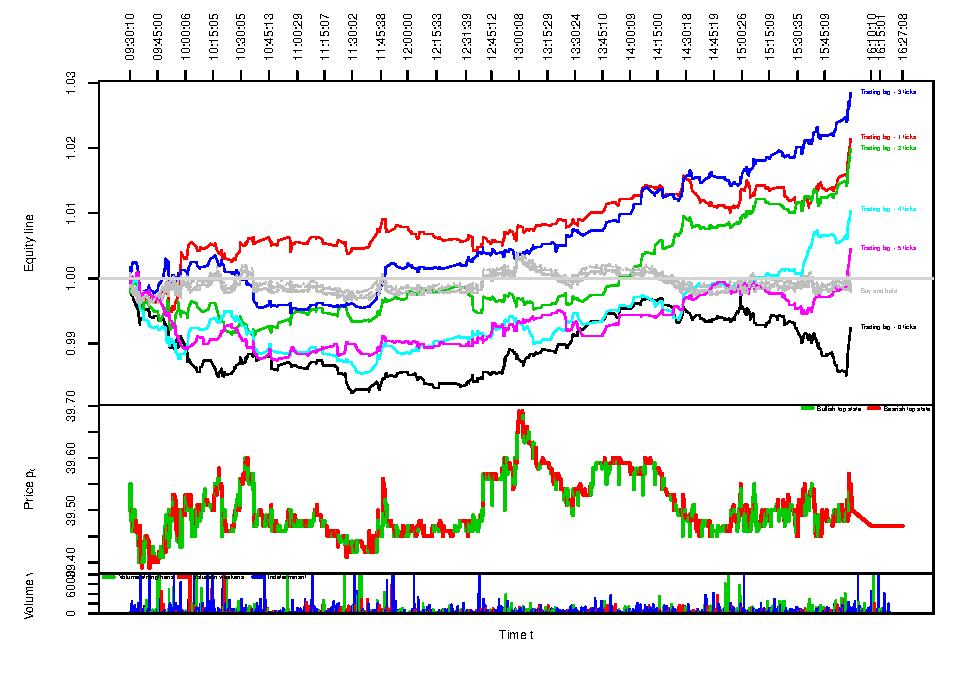
\includegraphics[width=\textwidth]{main_files/figure-latex/unnamed-chunk-28-1} \caption{Tick by tick sequence of trades, classified as belonging to the bear or the bull top state, from `r sym`.}\label{fig:unnamed-chunk-28}
\end{figure}

\newpage

\subsubsection{CTCa.TO}\label{ctca.to}

\begin{verbatim}
## Warning in par(cex.names = 0.7, cex.axis = 0.7, cex.lab = 0.7, cex.main =
## 0.7): "cex.names" is not a graphical parameter
\end{verbatim}

\begin{table}[h!]
\centering
\begingroup\scriptsize
\begin{tabularx}{\textwidth}{rRRRRRRR}
  \toprule
 & Buy-Hold & HHMM (0 lag) & HHMM (1 lag) & HHMM (2 lag) & HHMM (3 lag) & HHMM (4 lag) & HHMM (5 lag) \\ 
  \midrule
2007-05-08 & -0.01 & -0.00 & -0.00 & 0.00 & -0.01 & 0.00 & -0.00 \\ 
  2007-05-09 & -0.01 & -0.02 & -0.02 & -0.00 & 0.00 & 0.00 & -0.01 \\ 
  2007-05-10 & 0.05 & 0.03 & 0.02 & -0.01 & 0.03 & 0.04 & 0.06 \\ 
  2007-05-11 & 0.02 & 0.04 & 0.03 & 0.04 & 0.03 & 0.04 & 0.03 \\ 
  2007-05-14 & -0.00 & 0.04 & 0.01 & 0.00 & 0.02 & 0.00 & -0.01 \\ 
  2007-05-15 & 0.00 & -0.01 & -0.01 & 0.02 & 0.01 & 0.01 & -0.01 \\ 
  2007-05-16 & 0.02 & -0.02 & 0.01 & 0.02 & 0.02 & 0.01 & 0.04 \\ 
  2007-05-17 & 0.01 & 0.01 & 0.03 & 0.04 & 0.03 & 0.02 & 0.03 \\ 
  2007-05-18 & -0.01 & 0.02 & 0.02 & -0.00 & 0.00 & -0.01 & 0.00 \\ 
  2007-05-22 & 0.00 & 0.01 & -0.00 & -0.01 & 0.00 & 0.02 & 0.01 \\ 
  2007-05-23 & 0.01 & -0.01 & -0.01 & -0.00 & 0.01 & 0.02 & 0.00 \\ 
  2007-05-24 & -0.01 & -0.01 & -0.00 & 0.01 & 0.01 & 0.01 & 0.01 \\ 
  2007-05-25 & 0.01 & -0.00 & 0.02 & 0.01 & 0.00 & 0.01 & -0.01 \\ 
  2007-05-28 & 0.00 & 0.02 & -0.03 & 0.00 & 0.01 & 0.01 & 0.02 \\ 
  2007-05-29 & -0.01 & -0.01 & -0.01 & -0.01 & -0.01 & -0.00 & 0.02 \\ 
  2007-05-30 & 0.00 & 0.03 & 0.01 & -0.01 & -0.01 & -0.04 & -0.01 \\ 
  2007-05-31 & -0.00 & -0.01 & -0.02 & -0.02 & -0.03 & -0.00 & 0.01 \\ 
   \midrule
Total & 0.06 & 0.13 & 0.03 & 0.07 & 0.13 & 0.15 & 0.21 \\ 
   \bottomrule
\end{tabularx}
\endgroup
\caption{Compound daily return originated in the HHMM trading strategy for different levels of lags. Returns from the buy and hold strategy are included as a reference. Returns expressed in percentage. Lag measured in ticks between the end of the zig-zag and the execution of the trade (zero lag suffers from look-ahead bias). CTCa.TO} 
\label{tab:appendix-wf-CTCa.TO}
\end{table}

\begin{verbatim}
## Warning in par(cex.names = 0.7, cex.axis = 0.7, cex.lab = 0.7, cex.main =
## 0.7): "cex.names" is not a graphical parameter
\end{verbatim}

\begin{figure}[H]
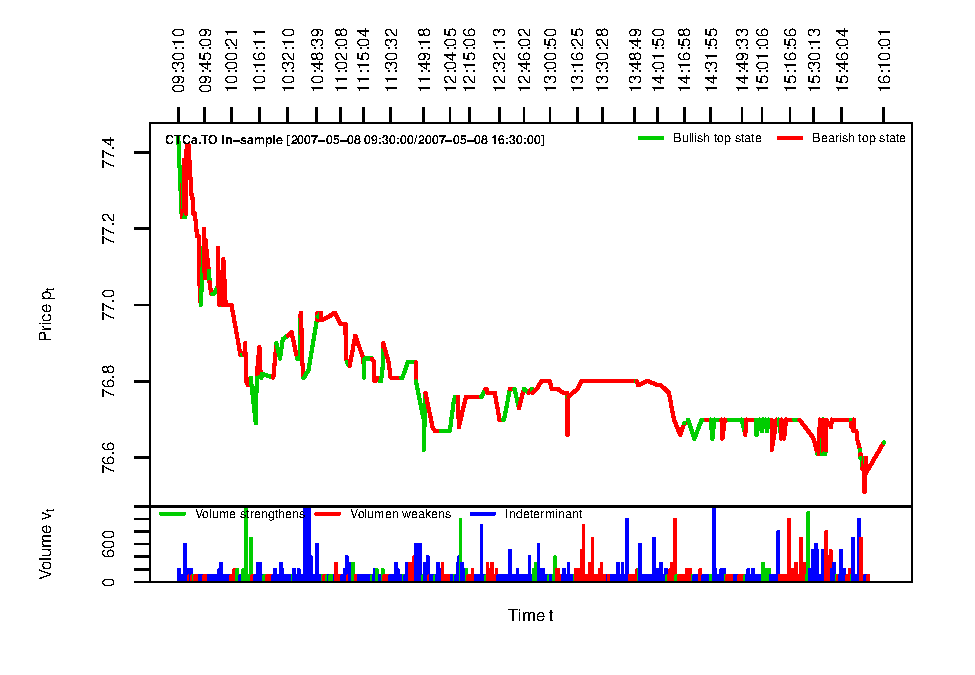
\includegraphics[width=\textwidth]{main_files/figure-latex/unnamed-chunk-30-1} \caption{Tick by tick sequence of trades, classified as belonging to the bear or the bull top state, from `r sym`.}\label{fig:unnamed-chunk-30}
\end{figure}

\newpage

\subsubsection{ECA.TO}\label{eca.to}

\begin{verbatim}
## Warning in par(cex.names = 0.7, cex.axis = 0.7, cex.lab = 0.7, cex.main =
## 0.7): "cex.names" is not a graphical parameter
\end{verbatim}

\begin{table}[h!]
\centering
\begingroup\scriptsize
\begin{tabularx}{\textwidth}{rRRRRRRR}
  \toprule
 & Buy-Hold & HHMM (0 lag) & HHMM (1 lag) & HHMM (2 lag) & HHMM (3 lag) & HHMM (4 lag) & HHMM (5 lag) \\ 
  \midrule
2007-05-08 & 0.01 & -0.01 & -0.02 & -0.02 & -0.01 & -0.01 & 0.01 \\ 
  2007-05-09 & -0.01 & -0.00 & -0.00 & 0.01 & 0.00 & -0.02 & 0.01 \\ 
  2007-05-10 & 0.00 & -0.01 & -0.04 & -0.04 & -0.03 & -0.04 & -0.03 \\ 
  2007-05-11 & 0.05 & 0.00 & -0.02 & -0.02 & 0.01 & -0.03 & -0.02 \\ 
  2007-05-14 & -0.01 & -0.02 & -0.01 & -0.00 & 0.00 & 0.02 & -0.02 \\ 
  2007-05-15 & 0.00 & 0.03 & -0.03 & -0.01 & -0.02 & -0.03 & -0.02 \\ 
  2007-05-16 & 0.02 & 0.02 & 0.03 & 0.03 & 0.02 & 0.02 & 0.01 \\ 
  2007-05-17 & 0.02 & 0.03 & 0.04 & 0.02 & 0.02 & 0.02 & 0.02 \\ 
  2007-05-18 & 0.00 & 0.02 & 0.02 & 0.02 & 0.01 & -0.00 & 0.03 \\ 
  2007-05-22 & -0.01 & -0.00 & 0.00 & -0.00 & -0.00 & -0.01 & -0.01 \\ 
  2007-05-23 & -0.01 & 0.01 & 0.01 & 0.00 & 0.01 & 0.02 & 0.02 \\ 
  2007-05-24 & -0.02 & -0.04 & -0.00 & 0.01 & 0.02 & 0.02 & 0.03 \\ 
  2007-05-25 & 0.00 & 0.04 & 0.05 & 0.03 & 0.03 & 0.02 & 0.02 \\ 
  2007-05-28 & -0.01 & 0.02 & 0.01 & 0.01 & 0.01 & 0.02 & -0.00 \\ 
  2007-05-29 & -0.01 & 0.04 & 0.01 & -0.00 & -0.01 & -0.02 & -0.03 \\ 
  2007-05-30 & 0.03 & 0.02 & 0.02 & -0.00 & 0.02 & 0.01 & 0.01 \\ 
  2007-05-31 & -0.01 & 0.06 & 0.02 & 0.02 & 0.03 & 0.03 & 0.01 \\ 
   \midrule
Total & 0.06 & 0.24 & 0.09 & 0.05 & 0.12 & 0.03 & 0.04 \\ 
   \bottomrule
\end{tabularx}
\endgroup
\caption{Compound daily return originated in the HHMM trading strategy for different levels of lags. Returns from the buy and hold strategy are included as a reference. Returns expressed in percentage. Lag measured in ticks between the end of the zig-zag and the execution of the trade (zero lag suffers from look-ahead bias). ECA.TO} 
\label{tab:appendix-wf-ECA.TO}
\end{table}

\begin{verbatim}
## Warning in par(cex.names = 0.7, cex.axis = 0.7, cex.lab = 0.7, cex.main =
## 0.7): "cex.names" is not a graphical parameter
\end{verbatim}

\begin{figure}[H]
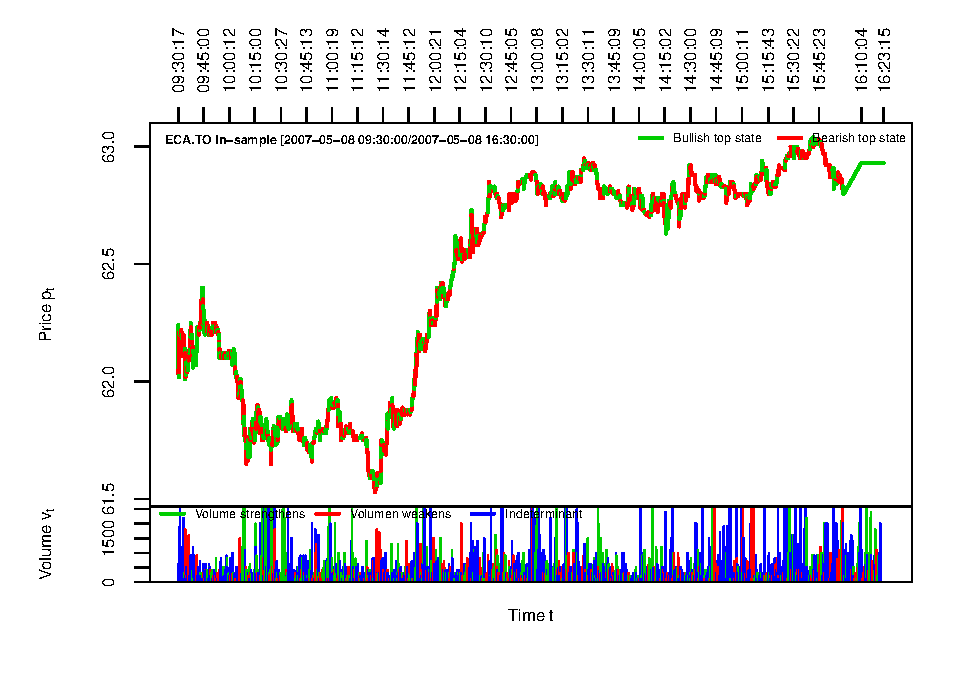
\includegraphics[width=\textwidth]{main_files/figure-latex/unnamed-chunk-32-1} \caption{Tick by tick sequence of trades, classified as belonging to the bear or the bull top state, from `r sym`.}\label{fig:unnamed-chunk-32}
\end{figure}

\newpage

\subsubsection{G.TO}\label{g.to}

\begin{verbatim}
## Warning in par(cex.names = 0.7, cex.axis = 0.7, cex.lab = 0.7, cex.main =
## 0.7): "cex.names" is not a graphical parameter
\end{verbatim}

\begin{table}[h!]
\centering
\begingroup\scriptsize
\begin{tabularx}{\textwidth}{rRRRRRRR}
  \toprule
 & Buy-Hold & HHMM (0 lag) & HHMM (1 lag) & HHMM (2 lag) & HHMM (3 lag) & HHMM (4 lag) & HHMM (5 lag) \\ 
  \midrule
2007-05-08 & -0.01 & 0.04 & -0.02 & -0.01 & 0.01 & 0.01 & 0.02 \\ 
  2007-05-09 & -0.00 & 0.04 & 0.00 & 0.02 & 0.02 & 0.01 & 0.01 \\ 
  2007-05-10 & -0.00 & 0.04 & 0.01 & -0.01 & 0.02 & 0.02 & 0.00 \\ 
  2007-05-11 & -0.00 & 0.00 & 0.00 & 0.01 & -0.00 & -0.01 & 0.00 \\ 
  2007-05-14 & -0.03 & 0.03 & -0.01 & 0.01 & -0.01 & -0.00 & -0.01 \\ 
  2007-05-15 & -0.00 & 0.03 & -0.00 & 0.00 & 0.02 & 0.02 & 0.00 \\ 
  2007-05-16 & -0.00 & 0.05 & -0.01 & -0.00 & 0.01 & 0.03 & -0.02 \\ 
  2007-05-17 & -0.00 & -0.02 & 0.00 & 0.02 & 0.00 & -0.03 & -0.00 \\ 
  2007-05-18 & 0.01 & -0.01 & 0.01 & 0.00 & 0.02 & 0.01 & 0.02 \\ 
  2007-05-22 & -0.02 & -0.02 & -0.02 & 0.02 & 0.01 & 0.02 & 0.02 \\ 
  2007-05-23 & -0.01 & 0.02 & -0.00 & -0.01 & -0.01 & 0.01 & 0.01 \\ 
  2007-05-24 & -0.03 & 0.02 & -0.00 & -0.01 & -0.01 & -0.00 & -0.02 \\ 
  2007-05-25 & 0.00 & -0.01 & -0.01 & 0.00 & 0.01 & -0.02 & -0.02 \\ 
  2007-05-28 & -0.01 & -0.02 & -0.01 & 0.01 & -0.01 & -0.01 & 0.02 \\ 
  2007-05-29 & -0.02 & -0.02 & -0.01 & -0.02 & -0.00 & 0.02 & 0.01 \\ 
  2007-05-30 & 0.01 & -0.02 & -0.03 & -0.03 & -0.01 & -0.04 & -0.02 \\ 
  2007-05-31 & 0.04 & 0.00 & -0.01 & -0.01 & -0.02 & -0.01 & -0.03 \\ 
   \midrule
Total & -0.09 & 0.17 & -0.12 & -0.01 & 0.04 & 0.02 & -0.02 \\ 
   \bottomrule
\end{tabularx}
\endgroup
\caption{Compound daily return originated in the HHMM trading strategy for different levels of lags. Returns from the buy and hold strategy are included as a reference. Returns expressed in percentage. Lag measured in ticks between the end of the zig-zag and the execution of the trade (zero lag suffers from look-ahead bias). G.TO} 
\label{tab:appendix-wf-G.TO}
\end{table}

\begin{verbatim}
## Warning in par(cex.names = 0.7, cex.axis = 0.7, cex.lab = 0.7, cex.main =
## 0.7): "cex.names" is not a graphical parameter
\end{verbatim}

\begin{figure}[H]
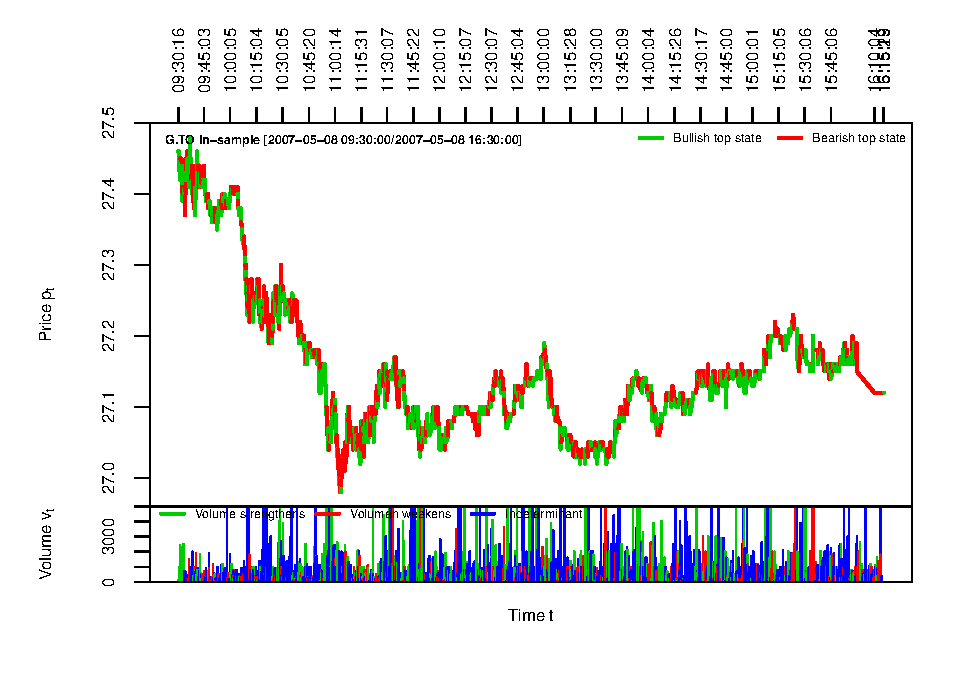
\includegraphics[width=\textwidth]{main_files/figure-latex/unnamed-chunk-34-1} \caption{Tick by tick sequence of trades, classified as belonging to the bear or the bull top state, from `r sym`.}\label{fig:unnamed-chunk-34}
\end{figure}

\newpage

\subsubsection{K.TO}\label{k.to}

\begin{verbatim}
## Warning in par(cex.names = 0.7, cex.axis = 0.7, cex.lab = 0.7, cex.main =
## 0.7): "cex.names" is not a graphical parameter
\end{verbatim}

\begin{table}[h!]
\centering
\begingroup\scriptsize
\begin{tabularx}{\textwidth}{rRRRRRRR}
  \toprule
 & Buy-Hold & HHMM (0 lag) & HHMM (1 lag) & HHMM (2 lag) & HHMM (3 lag) & HHMM (4 lag) & HHMM (5 lag) \\ 
  \midrule
2007-05-08 & -0.02 & -0.00 & -0.01 & 0.03 & 0.02 & 0.01 & 0.02 \\ 
  2007-05-09 & -0.01 & -0.05 & -0.04 & 0.01 & 0.02 & 0.01 & -0.00 \\ 
  2007-05-10 & -0.01 & 0.00 & 0.01 & 0.04 & 0.02 & 0.00 & -0.01 \\ 
  2007-05-11 & 0.01 & -0.02 & -0.05 & -0.03 & -0.00 & -0.02 & -0.01 \\ 
  2007-05-14 & -0.02 & 0.02 & 0.00 & 0.03 & 0.03 & 0.04 & -0.03 \\ 
  2007-05-15 & -0.01 & 0.05 & 0.01 & 0.04 & 0.04 & 0.03 & 0.02 \\ 
  2007-05-16 & -0.01 & 0.02 & -0.05 & -0.04 & -0.03 & -0.03 & -0.01 \\ 
  2007-05-17 & -0.00 & 0.01 & 0.01 & 0.03 & 0.03 & 0.03 & 0.01 \\ 
  2007-05-18 & 0.00 & -0.02 & -0.02 & -0.03 & 0.01 & 0.01 & 0.00 \\ 
  2007-05-22 & -0.02 & 0.01 & 0.00 & 0.01 & 0.01 & 0.02 & 0.01 \\ 
  2007-05-23 & 0.01 & -0.00 & -0.01 & -0.02 & 0.01 & 0.02 & -0.00 \\ 
  2007-05-24 & -0.03 & -0.10 & -0.08 & -0.07 & -0.02 & 0.01 & 0.01 \\ 
  2007-05-25 & -0.01 & -0.01 & 0.00 & -0.04 & -0.02 & -0.00 & 0.00 \\ 
  2007-05-28 & 0.00 & -0.00 & -0.01 & -0.00 & 0.01 & -0.01 & 0.01 \\ 
  2007-05-29 & -0.03 & -0.03 & 0.02 & 0.01 & 0.04 & 0.02 & 0.03 \\ 
  2007-05-30 & -0.00 & -0.00 & -0.03 & -0.02 & -0.01 & -0.01 & -0.01 \\ 
  2007-05-31 & 0.04 & 0.03 & -0.01 & -0.01 & -0.01 & -0.02 & -0.00 \\ 
   \midrule
Total & -0.10 & -0.11 & -0.22 & -0.07 & 0.14 & 0.12 & 0.03 \\ 
   \bottomrule
\end{tabularx}
\endgroup
\caption{Compound daily return originated in the HHMM trading strategy for different levels of lags. Returns from the buy and hold strategy are included as a reference. Returns expressed in percentage. Lag measured in ticks between the end of the zig-zag and the execution of the trade (zero lag suffers from look-ahead bias). K.TO} 
\label{tab:appendix-wf-K.TO}
\end{table}

\begin{verbatim}
## Warning in par(cex.names = 0.7, cex.axis = 0.7, cex.lab = 0.7, cex.main =
## 0.7): "cex.names" is not a graphical parameter
\end{verbatim}

\begin{figure}[H]
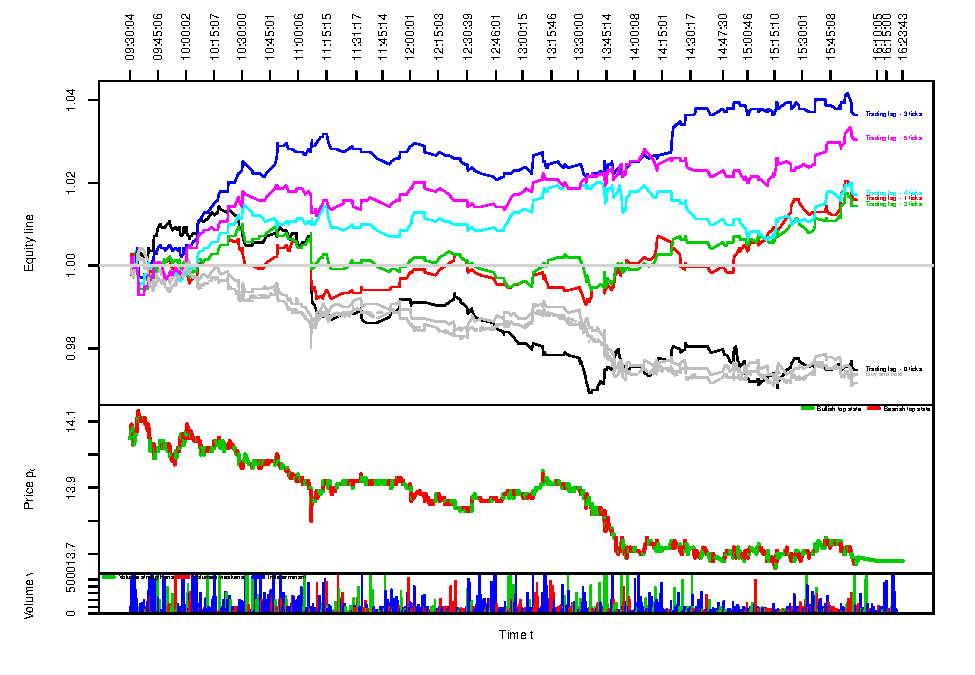
\includegraphics[width=\textwidth]{main_files/figure-latex/unnamed-chunk-36-1} \caption{Tick by tick sequence of trades, classified as belonging to the bear or the bull top state, from `r sym`.}\label{fig:unnamed-chunk-36}
\end{figure}

\newpage

\subsubsection{MGa.TO}\label{mga.to}

\begin{verbatim}
## Warning in par(cex.names = 0.7, cex.axis = 0.7, cex.lab = 0.7, cex.main =
## 0.7): "cex.names" is not a graphical parameter
\end{verbatim}

\begin{table}[h!]
\centering
\begingroup\scriptsize
\begin{tabularx}{\textwidth}{rRRRRRRR}
  \toprule
 & Buy-Hold & HHMM (0 lag) & HHMM (1 lag) & HHMM (2 lag) & HHMM (3 lag) & HHMM (4 lag) & HHMM (5 lag) \\ 
  \midrule
2007-05-08 & -0.02 & -0.05 & 0.00 & 0.02 & 0.04 & 0.01 & -0.01 \\ 
  2007-05-09 & 0.00 & -0.01 & -0.02 & -0.02 & 0.01 & 0.01 & 0.01 \\ 
  2007-05-10 & 0.06 & 0.21 & 0.13 & 0.11 & 0.08 & 0.01 & 0.01 \\ 
  2007-05-11 & 0.01 & 0.01 & 0.00 & -0.00 & -0.01 & -0.01 & 0.01 \\ 
  2007-05-14 & -0.03 & -0.03 & 0.01 & 0.01 & 0.02 & 0.03 & 0.01 \\ 
  2007-05-15 & -0.02 & 0.02 & -0.01 & 0.01 & 0.02 & -0.02 & -0.02 \\ 
  2007-05-16 & 0.01 & 0.02 & 0.00 & 0.01 & 0.01 & -0.01 & 0.00 \\ 
  2007-05-17 & -0.01 & 0.08 & 0.07 & 0.08 & 0.05 & 0.00 & 0.00 \\ 
  2007-05-18 & 0.01 & 0.03 & 0.04 & 0.03 & 0.02 & 0.03 & 0.02 \\ 
  2007-05-22 & 0.02 & 0.03 & 0.03 & 0.02 & 0.03 & 0.02 & 0.03 \\ 
  2007-05-23 & 0.01 & 0.05 & 0.03 & 0.01 & -0.01 & -0.02 & -0.00 \\ 
  2007-05-24 & 0.02 & -0.03 & 0.01 & 0.03 & 0.03 & 0.03 & 0.02 \\ 
  2007-05-25 & -0.00 & 0.00 & 0.01 & 0.02 & 0.01 & 0.00 & -0.01 \\ 
  2007-05-28 & 0.01 & 0.00 & 0.02 & 0.00 & -0.02 & -0.01 & -0.01 \\ 
  2007-05-29 & -0.01 & 0.01 & 0.00 & 0.01 & 0.00 & 0.01 & -0.02 \\ 
  2007-05-30 & 0.00 & 0.01 & 0.00 & -0.02 & -0.01 & 0.01 & -0.00 \\ 
  2007-05-31 & 0.01 & 0.06 & 0.04 & 0.03 & 0.03 & 0.03 & 0.02 \\ 
   \midrule
Total & 0.07 & 0.48 & 0.45 & 0.38 & 0.32 & 0.11 & 0.07 \\ 
   \bottomrule
\end{tabularx}
\endgroup
\caption{Compound daily return originated in the HHMM trading strategy for different levels of lags. Returns from the buy and hold strategy are included as a reference. Returns expressed in percentage. Lag measured in ticks between the end of the zig-zag and the execution of the trade (zero lag suffers from look-ahead bias). MGa.TO} 
\label{tab:appendix-wf-MGa.TO}
\end{table}

\begin{verbatim}
## Warning in par(cex.names = 0.7, cex.axis = 0.7, cex.lab = 0.7, cex.main =
## 0.7): "cex.names" is not a graphical parameter
\end{verbatim}

\begin{figure}[H]
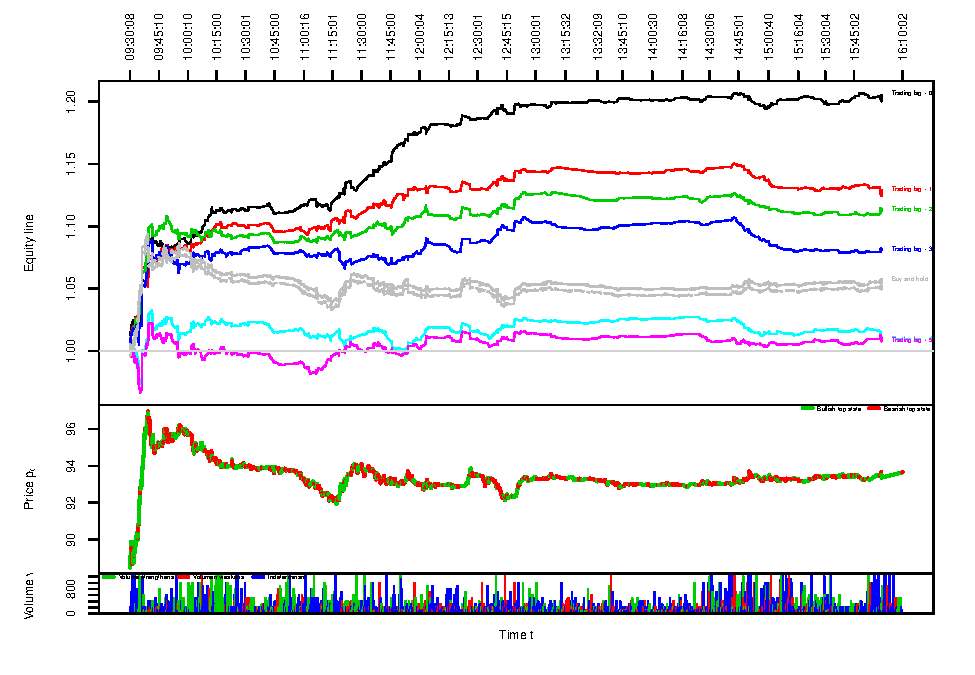
\includegraphics[width=\textwidth]{main_files/figure-latex/unnamed-chunk-38-1} \caption{Tick by tick sequence of trades, classified as belonging to the bear or the bull top state, from `r sym`.}\label{fig:unnamed-chunk-38}
\end{figure}

\newpage

\subsubsection{NXY.TO}\label{nxy.to}

\begin{verbatim}
## Warning in par(cex.names = 0.7, cex.axis = 0.7, cex.lab = 0.7, cex.main =
## 0.7): "cex.names" is not a graphical parameter
\end{verbatim}

\begin{table}[h!]
\centering
\begingroup\scriptsize
\begin{tabularx}{\textwidth}{rRRRRRRR}
  \toprule
 & Buy-Hold & HHMM (0 lag) & HHMM (1 lag) & HHMM (2 lag) & HHMM (3 lag) & HHMM (4 lag) & HHMM (5 lag) \\ 
  \midrule
2007-05-08 & 0.00 & 0.05 & -0.01 & 0.02 & 0.01 & 0.00 & 0.01 \\ 
  2007-05-09 & -0.01 & 0.04 & 0.03 & 0.03 & 0.04 & 0.04 & 0.04 \\ 
  2007-05-10 & -0.01 & -0.07 & -0.04 & -0.01 & 0.02 & -0.01 & 0.03 \\ 
  2007-05-11 & 0.02 & -0.00 & -0.04 & -0.02 & -0.00 & -0.00 & 0.01 \\ 
  2007-05-14 & -0.02 & -0.04 & -0.00 & 0.01 & 0.02 & 0.02 & 0.04 \\ 
  2007-05-15 & -0.01 & -0.01 & -0.02 & -0.01 & -0.00 & -0.00 & -0.01 \\ 
  2007-05-16 & 0.02 & -0.01 & -0.00 & -0.03 & 0.03 & 0.06 & 0.03 \\ 
  2007-05-17 & 0.02 & 0.03 & 0.00 & -0.00 & -0.01 & -0.02 & -0.02 \\ 
  2007-05-18 & -0.01 & -0.04 & -0.06 & -0.06 & -0.03 & -0.00 & 0.01 \\ 
  2007-05-22 & -0.02 & 0.01 & 0.01 & -0.01 & 0.01 & 0.01 & 0.01 \\ 
  2007-05-23 & -0.01 & 0.02 & 0.01 & 0.01 & 0.01 & 0.04 & 0.02 \\ 
  2007-05-24 & -0.03 & 0.03 & 0.02 & 0.00 & 0.02 & 0.03 & 0.01 \\ 
  2007-05-25 & -0.02 & -0.01 & -0.05 & -0.03 & -0.01 & -0.01 & -0.01 \\ 
  2007-05-28 & 0.00 & 0.01 & 0.01 & 0.02 & 0.03 & 0.02 & 0.02 \\ 
  2007-05-29 & -0.00 & -0.00 & -0.01 & -0.01 & 0.01 & -0.01 & -0.02 \\ 
  2007-05-30 & 0.02 & -0.01 & -0.00 & 0.02 & 0.01 & 0.01 & -0.03 \\ 
  2007-05-31 & -0.01 & 0.02 & -0.00 & -0.00 & 0.01 & -0.00 & 0.00 \\ 
   \midrule
Total & -0.07 & 0.01 & -0.16 & -0.08 & 0.18 & 0.17 & 0.14 \\ 
   \bottomrule
\end{tabularx}
\endgroup
\caption{Compound daily return originated in the HHMM trading strategy for different levels of lags. Returns from the buy and hold strategy are included as a reference. Returns expressed in percentage. Lag measured in ticks between the end of the zig-zag and the execution of the trade (zero lag suffers from look-ahead bias). NXY.TO} 
\label{tab:appendix-wf-NXY.TO}
\end{table}

\begin{verbatim}
## Warning in par(cex.names = 0.7, cex.axis = 0.7, cex.lab = 0.7, cex.main =
## 0.7): "cex.names" is not a graphical parameter
\end{verbatim}

\begin{figure}[H]
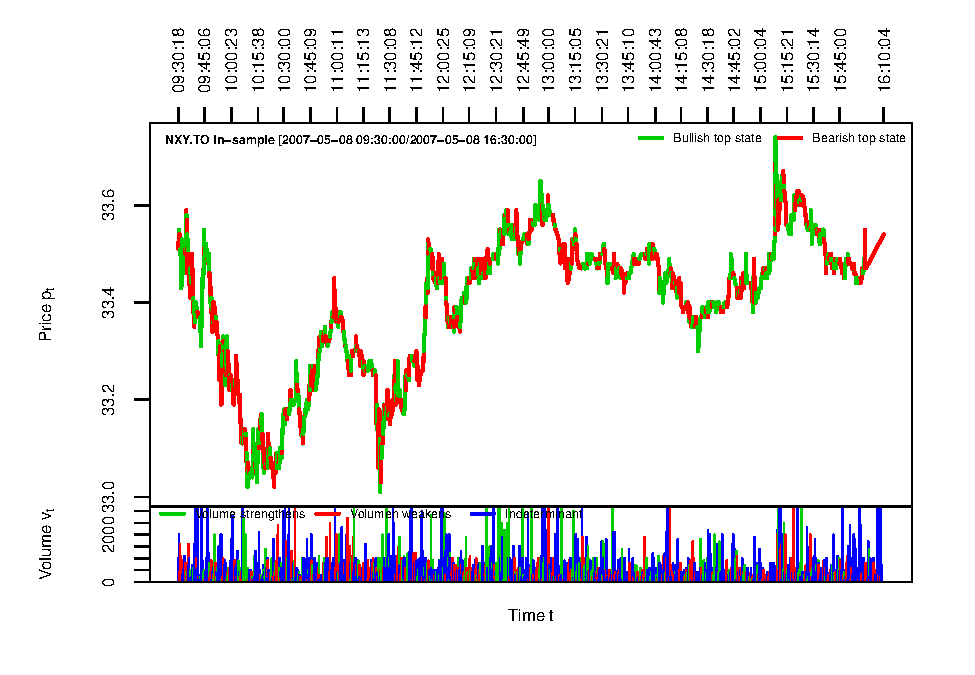
\includegraphics[width=\textwidth]{main_files/figure-latex/unnamed-chunk-40-1} \caption{Tick by tick sequence of trades, classified as belonging to the bear or the bull top state, from `r sym`.}\label{fig:unnamed-chunk-40}
\end{figure}

\newpage

\subsubsection{SJRb.TO}\label{sjrb.to}

\begin{verbatim}
## Warning in par(cex.names = 0.7, cex.axis = 0.7, cex.lab = 0.7, cex.main =
## 0.7): "cex.names" is not a graphical parameter
\end{verbatim}

\begin{table}[h!]
\centering
\begingroup\scriptsize
\begin{tabularx}{\textwidth}{rRRRRRRR}
  \toprule
 & Buy-Hold & HHMM (0 lag) & HHMM (1 lag) & HHMM (2 lag) & HHMM (3 lag) & HHMM (4 lag) & HHMM (5 lag) \\ 
  \midrule
2007-05-08 & 0.00 & 0.01 & 0.01 & 0.03 & 0.02 & -0.00 & 0.01 \\ 
  2007-05-09 & -0.02 & 0.01 & 0.01 & -0.03 & -0.02 & -0.01 & 0.00 \\ 
  2007-05-10 & 0.00 & -0.04 & -0.07 & -0.06 & -0.04 & -0.02 & -0.06 \\ 
  2007-05-11 & 0.02 & -0.05 & -0.03 & -0.02 & -0.00 & -0.01 & 0.02 \\ 
  2007-05-14 & -0.02 & -0.02 & -0.02 & 0.01 & -0.00 & 0.00 & -0.01 \\ 
  2007-05-15 & -0.00 & 0.00 & -0.01 & 0.00 & -0.01 & -0.02 & -0.02 \\ 
  2007-05-16 & 0.02 & 0.01 & 0.01 & -0.01 & -0.01 & -0.01 & -0.02 \\ 
  2007-05-17 & 0.01 & 0.01 & -0.02 & -0.00 & 0.01 & -0.01 & 0.01 \\ 
  2007-05-18 & 0.00 & -0.05 & 0.02 & -0.01 & -0.01 & 0.01 & -0.01 \\ 
  2007-05-22 & -0.01 & -0.04 & -0.03 & -0.03 & -0.03 & -0.02 & -0.02 \\ 
  2007-05-23 & 0.01 & 0.02 & 0.01 & 0.04 & 0.03 & 0.01 & 0.01 \\ 
  2007-05-24 & -0.02 & -0.04 & -0.02 & -0.00 & -0.01 & -0.02 & -0.01 \\ 
  2007-05-25 & -0.00 & 0.01 & 0.03 & 0.02 & -0.01 & 0.00 & -0.00 \\ 
  2007-05-28 & -0.00 & 0.02 & 0.03 & 0.02 & 0.01 & 0.04 & 0.02 \\ 
  2007-05-29 & 0.01 & -0.02 & -0.01 & -0.05 & 0.00 & -0.00 & -0.01 \\ 
  2007-05-30 & 0.01 & 0.01 & 0.02 & 0.01 & 0.00 & 0.02 & 0.01 \\ 
  2007-05-31 & -0.01 & -0.03 & -0.02 & 0.01 & -0.01 & -0.01 & -0.03 \\ 
   \midrule
Total & 0.01 & -0.18 & -0.06 & -0.06 & -0.06 & -0.05 & -0.11 \\ 
   \bottomrule
\end{tabularx}
\endgroup
\caption{Compound daily return originated in the HHMM trading strategy for different levels of lags. Returns from the buy and hold strategy are included as a reference. Returns expressed in percentage. Lag measured in ticks between the end of the zig-zag and the execution of the trade (zero lag suffers from look-ahead bias). SJRb.TO} 
\label{tab:appendix-wf-SJRb.TO}
\end{table}

\begin{verbatim}
## Warning in par(cex.names = 0.7, cex.axis = 0.7, cex.lab = 0.7, cex.main =
## 0.7): "cex.names" is not a graphical parameter
\end{verbatim}

\begin{figure}[H]
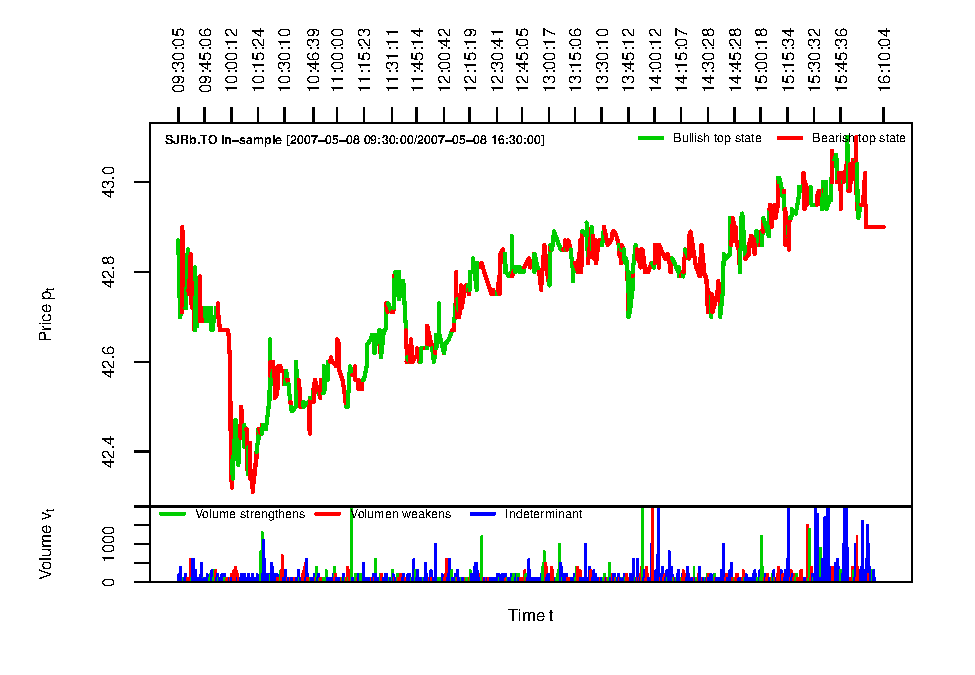
\includegraphics[width=\textwidth]{main_files/figure-latex/unnamed-chunk-42-1} \caption{Tick by tick sequence of trades, classified as belonging to the bear or the bull top state, from `r sym`.}\label{fig:unnamed-chunk-42}
\end{figure}

\newpage

\subsubsection{SU.TO}\label{su.to}

\begin{verbatim}
## Warning in par(cex.names = 0.7, cex.axis = 0.7, cex.lab = 0.7, cex.main =
## 0.7): "cex.names" is not a graphical parameter
\end{verbatim}

\begin{table}[h!]
\centering
\begingroup\scriptsize
\begin{tabularx}{\textwidth}{rRRRRRRR}
  \toprule
 & Buy-Hold & HHMM (0 lag) & HHMM (1 lag) & HHMM (2 lag) & HHMM (3 lag) & HHMM (4 lag) & HHMM (5 lag) \\ 
  \midrule
2007-05-08 & 0.01 & 0.00 & 0.02 & 0.00 & 0.01 & 0.00 & 0.01 \\ 
  2007-05-09 & 0.01 & 0.04 & -0.02 & -0.01 & 0.01 & 0.01 & -0.01 \\ 
  2007-05-10 & -0.01 & 0.01 & 0.01 & 0.02 & 0.02 & -0.01 & -0.02 \\ 
  2007-05-11 & 0.02 & 0.02 & 0.02 & 0.02 & -0.00 & -0.01 & -0.01 \\ 
  2007-05-14 & -0.00 & 0.01 & -0.01 & -0.01 & -0.01 & -0.01 & 0.01 \\ 
  2007-05-15 & -0.02 & 0.02 & 0.01 & -0.02 & -0.01 & -0.02 & -0.02 \\ 
  2007-05-16 & 0.02 & 0.01 & 0.02 & 0.01 & -0.01 & 0.01 & 0.01 \\ 
  2007-05-17 & 0.03 & 0.04 & 0.04 & 0.03 & 0.02 & 0.02 & 0.03 \\ 
  2007-05-18 & 0.01 & 0.02 & -0.01 & -0.01 & -0.00 & -0.01 & -0.01 \\ 
  2007-05-22 & -0.00 & 0.05 & 0.01 & 0.01 & 0.02 & 0.02 & 0.02 \\ 
  2007-05-23 & 0.01 & -0.00 & 0.00 & 0.01 & 0.00 & 0.02 & 0.03 \\ 
  2007-05-24 & -0.03 & 0.04 & 0.04 & 0.03 & 0.02 & 0.04 & -0.01 \\ 
  2007-05-25 & 0.01 & 0.02 & 0.00 & 0.00 & -0.01 & 0.01 & 0.01 \\ 
  2007-05-28 & 0.00 & 0.01 & 0.01 & -0.01 & -0.01 & -0.00 & -0.01 \\ 
  2007-05-29 & -0.02 & 0.01 & -0.03 & -0.02 & -0.00 & -0.01 & -0.01 \\ 
  2007-05-30 & 0.01 & 0.04 & 0.02 & 0.01 & -0.02 & 0.00 & 0.01 \\ 
  2007-05-31 & 0.00 & 0.04 & 0.03 & 0.03 & 0.02 & 0.02 & 0.02 \\ 
   \midrule
Total & 0.03 & 0.45 & 0.18 & 0.08 & 0.04 & 0.09 & 0.05 \\ 
   \bottomrule
\end{tabularx}
\endgroup
\caption{Compound daily return originated in the HHMM trading strategy for different levels of lags. Returns from the buy and hold strategy are included as a reference. Returns expressed in percentage. Lag measured in ticks between the end of the zig-zag and the execution of the trade (zero lag suffers from look-ahead bias). SU.TO} 
\label{tab:appendix-wf-SU.TO}
\end{table}

\begin{verbatim}
## Warning in par(cex.names = 0.7, cex.axis = 0.7, cex.lab = 0.7, cex.main =
## 0.7): "cex.names" is not a graphical parameter
\end{verbatim}

\begin{figure}[H]
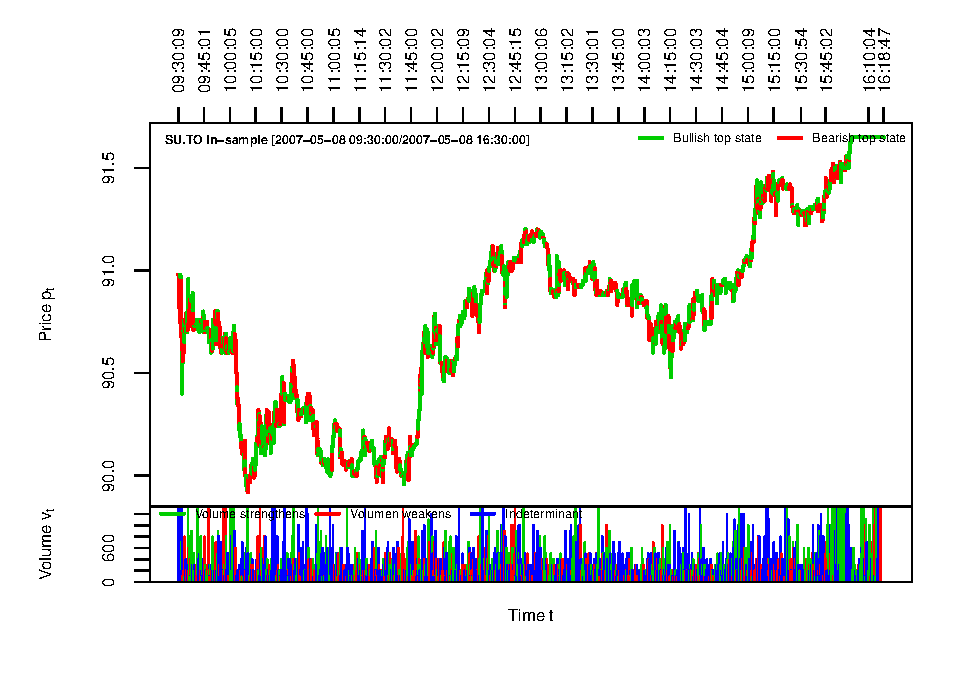
\includegraphics[width=\textwidth]{main_files/figure-latex/unnamed-chunk-44-1} \caption{Tick by tick sequence of trades, classified as belonging to the bear or the bull top state, from `r sym`.}\label{fig:unnamed-chunk-44}
\end{figure}

\newpage

\subsubsection{TCKb.TO}\label{tckb.to}

\begin{verbatim}
## Warning in par(cex.names = 0.7, cex.axis = 0.7, cex.lab = 0.7, cex.main =
## 0.7): "cex.names" is not a graphical parameter
\end{verbatim}

\begin{table}[h!]
\centering
\begingroup\scriptsize
\begin{tabularx}{\textwidth}{rRRRRRRR}
  \toprule
 & Buy-Hold & HHMM (0 lag) & HHMM (1 lag) & HHMM (2 lag) & HHMM (3 lag) & HHMM (4 lag) & HHMM (5 lag) \\ 
  \midrule
2007-05-08 & -0.01 & -0.00 & -0.01 & -0.00 & -0.00 & 0.01 & 0.02 \\ 
  2007-05-09 & 0.02 & -0.00 & -0.02 & 0.01 & 0.04 & 0.04 & -0.00 \\ 
  2007-05-10 & 0.01 & 0.01 & 0.02 & 0.06 & 0.05 & 0.04 & 0.03 \\ 
  2007-05-11 & 0.03 & -0.02 & -0.00 & -0.01 & 0.01 & 0.01 & -0.02 \\ 
  2007-05-14 & -0.05 & 0.00 & -0.03 & -0.05 & -0.02 & -0.01 & -0.03 \\ 
  2007-05-15 & -0.00 & 0.05 & -0.01 & 0.01 & 0.03 & 0.03 & 0.03 \\ 
  2007-05-16 & -0.01 & -0.03 & -0.03 & -0.01 & -0.04 & -0.02 & 0.01 \\ 
  2007-05-17 & 0.00 & 0.08 & -0.03 & -0.04 & -0.03 & -0.03 & 0.00 \\ 
  2007-05-18 & 0.01 & 0.02 & 0.01 & 0.01 & 0.01 & 0.03 & -0.00 \\ 
  2007-05-22 & -0.04 & 0.01 & 0.00 & 0.02 & 0.02 & 0.02 & 0.02 \\ 
  2007-05-23 & -0.01 & -0.02 & -0.01 & -0.01 & -0.01 & 0.01 & -0.01 \\ 
  2007-05-24 & -0.04 & 0.06 & 0.04 & 0.04 & 0.02 & 0.02 & 0.04 \\ 
  2007-05-25 & 0.01 & 0.02 & -0.02 & -0.02 & -0.03 & -0.01 & -0.01 \\ 
  2007-05-28 & 0.01 & -0.01 & -0.01 & 0.01 & 0.01 & -0.00 & 0.00 \\ 
  2007-05-29 & -0.02 & -0.00 & -0.02 & -0.01 & -0.00 & -0.00 & 0.00 \\ 
  2007-05-30 & 0.04 & 0.09 & 0.05 & 0.07 & 0.06 & 0.08 & 0.05 \\ 
  2007-05-31 & 0.00 & 0.02 & 0.01 & 0.03 & -0.01 & 0.00 & -0.01 \\ 
   \midrule
Total & -0.06 & 0.29 & -0.06 & 0.11 & 0.10 & 0.23 & 0.12 \\ 
   \bottomrule
\end{tabularx}
\endgroup
\caption{Compound daily return originated in the HHMM trading strategy for different levels of lags. Returns from the buy and hold strategy are included as a reference. Returns expressed in percentage. Lag measured in ticks between the end of the zig-zag and the execution of the trade (zero lag suffers from look-ahead bias). TCKb.TO} 
\label{tab:appendix-wf-TCKb.TO}
\end{table}

\begin{verbatim}
## Warning in par(cex.names = 0.7, cex.axis = 0.7, cex.lab = 0.7, cex.main =
## 0.7): "cex.names" is not a graphical parameter
\end{verbatim}

\begin{figure}[H]
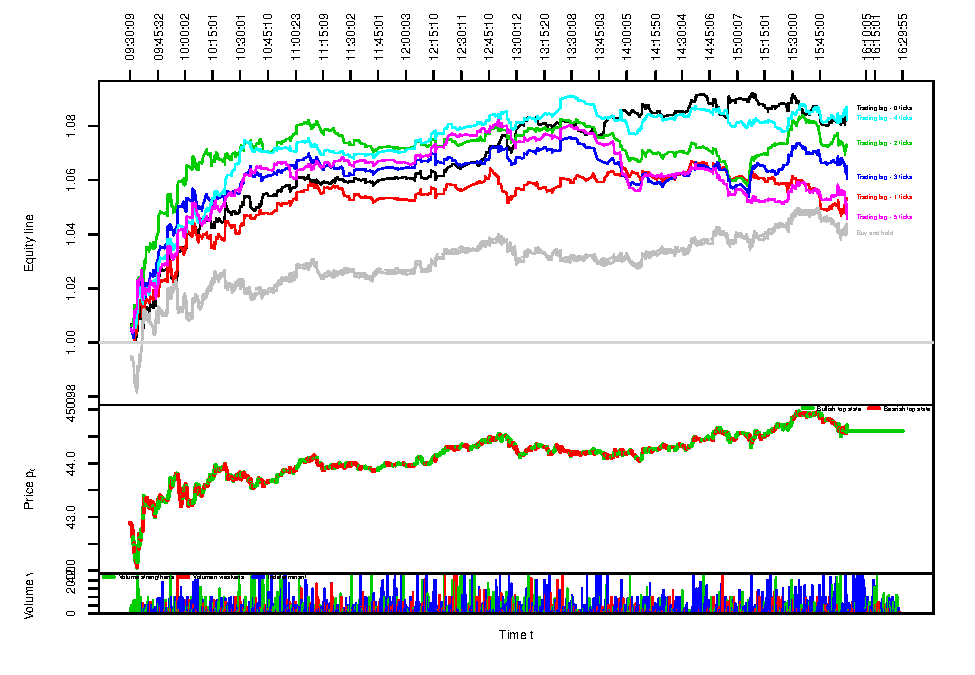
\includegraphics[width=\textwidth]{main_files/figure-latex/unnamed-chunk-46-1} \caption{Tick by tick sequence of trades, classified as belonging to the bear or the bull top state, from `r sym`.}\label{fig:unnamed-chunk-46}
\end{figure}

\newpage

\subsubsection{TLM.TO}\label{tlm.to}

\begin{verbatim}
## Warning in par(cex.names = 0.7, cex.axis = 0.7, cex.lab = 0.7, cex.main =
## 0.7): "cex.names" is not a graphical parameter
\end{verbatim}

\begin{table}[h!]
\centering
\begingroup\scriptsize
\begin{tabularx}{\textwidth}{rRRRRRRR}
  \toprule
 & Buy-Hold & HHMM (0 lag) & HHMM (1 lag) & HHMM (2 lag) & HHMM (3 lag) & HHMM (4 lag) & HHMM (5 lag) \\ 
  \midrule
2007-05-08 & 0.01 & 0.03 & -0.00 & -0.02 & -0.01 & -0.01 & -0.01 \\ 
  2007-05-09 & -0.03 & 0.01 & -0.00 & -0.01 & 0.00 & 0.03 & 0.01 \\ 
  2007-05-10 & -0.02 & 0.00 & -0.01 & -0.02 & 0.00 & -0.00 & 0.01 \\ 
  2007-05-11 & 0.03 & -0.02 & -0.03 & -0.01 & -0.01 & -0.00 & -0.00 \\ 
  2007-05-14 & -0.00 & -0.00 & 0.01 & -0.01 & 0.01 & 0.00 & -0.02 \\ 
  2007-05-15 & -0.01 & -0.01 & -0.01 & -0.03 & -0.01 & -0.01 & -0.01 \\ 
  2007-05-16 & 0.01 & 0.01 & 0.02 & 0.01 & 0.02 & 0.02 & 0.00 \\ 
  2007-05-17 & 0.02 & -0.01 & 0.01 & -0.01 & -0.01 & -0.01 & -0.00 \\ 
  2007-05-18 & -0.00 & -0.05 & -0.01 & -0.01 & -0.01 & -0.01 & 0.01 \\ 
  2007-05-22 & -0.01 & -0.01 & -0.02 & -0.02 & -0.02 & -0.02 & -0.01 \\ 
  2007-05-23 & 0.01 & 0.01 & -0.02 & -0.02 & -0.00 & 0.02 & 0.01 \\ 
  2007-05-24 & -0.02 & -0.00 & 0.02 & 0.02 & 0.01 & 0.02 & 0.04 \\ 
  2007-05-25 & 0.00 & -0.02 & -0.00 & 0.02 & 0.01 & 0.01 & 0.01 \\ 
  2007-05-28 & 0.01 & -0.02 & -0.01 & 0.00 & -0.01 & 0.00 & -0.01 \\ 
  2007-05-29 & -0.02 & 0.01 & 0.01 & 0.02 & -0.02 & 0.00 & 0.01 \\ 
  2007-05-30 & 0.04 & -0.01 & 0.01 & 0.03 & 0.01 & -0.01 & 0.01 \\ 
  2007-05-31 & -0.02 & -0.02 & 0.01 & -0.03 & -0.02 & 0.00 & 0.00 \\ 
   \midrule
Total & -0.02 & -0.09 & -0.03 & -0.10 & -0.05 & 0.04 & 0.07 \\ 
   \bottomrule
\end{tabularx}
\endgroup
\caption{Compound daily return originated in the HHMM trading strategy for different levels of lags. Returns from the buy and hold strategy are included as a reference. Returns expressed in percentage. Lag measured in ticks between the end of the zig-zag and the execution of the trade (zero lag suffers from look-ahead bias). TLM.TO} 
\label{tab:appendix-wf-TLM.TO}
\end{table}

\begin{verbatim}
## Warning in par(cex.names = 0.7, cex.axis = 0.7, cex.lab = 0.7, cex.main =
## 0.7): "cex.names" is not a graphical parameter
\end{verbatim}

\begin{figure}[H]
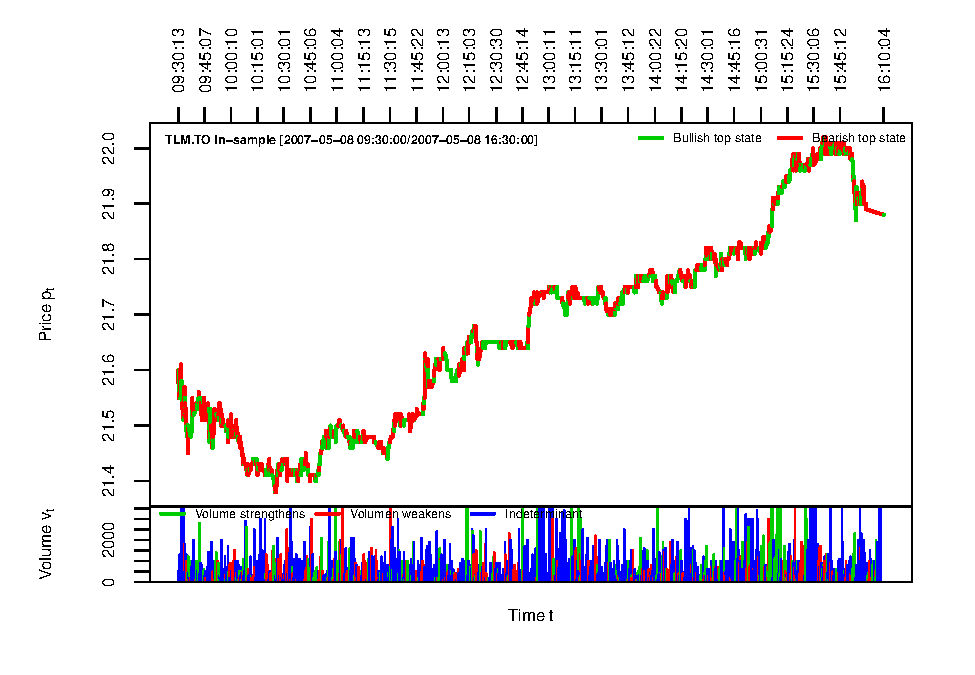
\includegraphics[width=\textwidth]{main_files/figure-latex/unnamed-chunk-48-1} \caption{Tick by tick sequence of trades, classified as belonging to the bear or the bull top state, from `r sym`.}\label{fig:unnamed-chunk-48}
\end{figure}

\newpage

\subsection{Original Computing
Environment}\label{original-computing-environment}

\begin{verbatim}
## 
## CXXFLAGS=-O3 -mtune=native -march=native -Wno-unused-variable -Wno-unused-function
\end{verbatim}

\begin{verbatim}
## Session info -------------------------------------------------------------
\end{verbatim}

\begin{verbatim}
##  setting  value                       
##  version  R version 3.3.3 (2017-03-06)
##  system   x86_64, mingw32             
##  ui       RTerm                       
##  language (EN)                        
##  collate  Spanish_Argentina.1252      
##  tz       America/Buenos_Aires        
##  date     2017-08-27
\end{verbatim}

\begin{verbatim}
## Packages -----------------------------------------------------------------
\end{verbatim}

\begin{verbatim}
##  package      * version   date       source        
##  BH             1.62.0-1  2016-11-19 CRAN (R 3.3.2)
##  colorspace     1.3-2     2016-12-14 CRAN (R 3.3.3)
##  dichromat      2.0-0     2013-01-24 CRAN (R 3.3.2)
##  digest       * 0.6.12    2017-01-27 CRAN (R 3.3.3)
##  ggplot2      * 2.2.1     2016-12-30 CRAN (R 3.3.3)
##  graphics     * 3.3.3     2017-03-06 local         
##  grDevices    * 3.3.3     2017-03-06 local         
##  grid           3.3.3     2017-03-06 local         
##  gridExtra      2.2.1     2016-02-29 CRAN (R 3.3.3)
##  gtable         0.2.0     2016-02-26 CRAN (R 3.3.3)
##  inline         0.3.14    2015-04-13 CRAN (R 3.3.3)
##  labeling       0.3       2014-08-23 CRAN (R 3.3.2)
##  lattice        0.20-34   2016-09-06 CRAN (R 3.3.3)
##  lazyeval       0.2.0     2016-06-12 CRAN (R 3.3.3)
##  magrittr       1.5       2014-11-22 CRAN (R 3.3.3)
##  MASS           7.3-45    2016-04-21 CRAN (R 3.3.3)
##  Matrix         1.2-8     2017-01-20 CRAN (R 3.3.3)
##  methods      * 3.3.3     2017-03-06 local         
##  munsell        0.4.3     2016-02-13 CRAN (R 3.3.3)
##  plyr           1.8.4     2016-06-08 CRAN (R 3.3.3)
##  RColorBrewer   1.1-2     2014-12-07 CRAN (R 3.3.2)
##  Rcpp           0.12.10   2017-03-19 CRAN (R 3.3.3)
##  RcppEigen      0.3.2.9.1 2017-03-15 CRAN (R 3.3.3)
##  reshape2       1.4.2     2016-10-22 CRAN (R 3.3.3)
##  rstan        * 2.14.2    2017-03-19 CRAN (R 3.3.3)
##  scales         0.4.1     2016-11-09 CRAN (R 3.3.3)
##  StanHeaders  * 2.14.0-1  2017-01-09 CRAN (R 3.3.3)
##  stats        * 3.3.3     2017-03-06 local         
##  stats4         3.3.3     2017-03-06 local         
##  stringi        1.1.3     2017-03-21 CRAN (R 3.3.3)
##  stringr        1.2.0     2017-02-18 CRAN (R 3.3.3)
##  tibble         1.3.0     2017-04-01 CRAN (R 3.3.3)
##  tools          3.3.3     2017-03-06 local         
##  utils        * 3.3.3     2017-03-06 local
\end{verbatim}


\end{document}
